\documentclass[a4paper]{article}

%% Language and font encodings
\usepackage[english]{babel}
\usepackage[utf8]{inputenc}
\usepackage[T1]{fontenc}

%% AW ADDED:
\usepackage{soul} % good for highlighting and underlining text
\usepackage[notref,notcite]{showkeys} % equation labels appear next to equations 

%% Sets page size and margins
\usepackage[a4paper,top=3cm,bottom=2cm,left=3cm,right=3cm,marginparwidth=1.75cm]{geometry}

%% Useful packages
\usepackage{amsmath}
\usepackage{amsfonts}
\usepackage{graphicx}
\usepackage[colorinlistoftodos]{todonotes}
\usepackage[colorlinks=true, allcolors=blue]{hyperref}
\usepackage{subfig}
\usepackage{xcolor}

% bibliography
\usepackage[backend=bibtex,style=numeric,citestyle=numeric,maxbibnames=99]{biblatex}
\renewbibmacro{in:}{\ifentrytype{article}{}{\printtext{\bibstring{in}\intitlepunct}}}
\bibliography{DoMath_bibliography.bib}

% AW added
\newcommand{\ip}[2]{\ensuremath{ \left< \left. #1 \right| #2 \right> } } % nice command to make an inner product

\newcommand{\aw}[1]{{\color{blue} [AW: #1]}}
\newcommand{\jm}[1]{{\color{red} [JM: #1]}}
\newcommand{\ap}[1]{{\color{red} [AP: #1]}}

\title{Edge states in disordered media and the Clifford pseudo-spectrum of three almost-commuting matrices \footnote{ \aw{Changed from ``non-periodic edge states''. The edge states may be periodic; the point is that we are studying such states in a medium (material) which is not. The term ``disordered'' is appropriate: it is not just that the pattern of the medium doesn't repeat itself, the material actually has no order: seeing what the material looks like in one place doesn't tell you very much about what it looks like in another because the atomic positions and onsite potentials are random. In, for example, a ``quasi-crystal'' the structure of the medium is ordered in the sense that it can be generated by a deterministic algorithm. This is not true for the media we are considering.} } }
\author{Jonathan Michala and Alexander Pierson}

\begin{document}

\aw{some things I want to make a note of:} 
\begin{itemize}
\item We have to make the bibliography: I can show you how to do this (it's a pain) using BibDesk \aw{this is an edit}
\item Deadline for report is December 17th (the last day of finals)
\item Bibliography test: A good book for solid state physics is \cite{1976AshcroftMermin}.
\item A couple of things which need to be worked out at some point (*after* we submit this writeup):
\begin{itemize}
\item In addition to mapping out the ``local index'' at each point, we should map out the size of the ``local gap'': the size of the smallest eigenvalue of the matrix $B$. This should give us a sense of when the edge states will actually be stable.
\item When we consider disorder of the atom positions, we should replace $t \rightarrow t e^{1 - r/r_0}$ where $r$ is the distance between atoms and $r_0$ is the distance between atoms *without disorder* and do the same for complex hopping too.
\item We should also consider the effect of the localization parameter
\end{itemize}
\end{itemize}
\aw{Nature of final report from Duke math website:} \\

Nature of Final Product \\

The final product for your research independent study will be a formal paper (as opposed to an informal report) that meets the criteria listed below. \\

1. The paper describes important aspects of the work done during the course. \\

2. The paper is thoughtful, well organized, and well written. It should be carefully proofread. \\

3. The paper communicates well to as broad an audience as would reasonably be assumed to have interest in your research topic. \\

4. The first part of the paper (two pages minimum) describes the broader context in which the project took place. This section should be written in a way that is understandable to an individual who has no specialized knowledge beyond the standard course content regularly offered by the Duke math department. \\

Specialized technical terms should be defined or avoided. \\

If your project involved a particular problem in a field of pure mathematics, it should be related to broader questions within that field. \\

If your project involved an application of mathematics, appropriate background material should be explained to motivate the problem and set it in a suitable context. \\

If non-standard mathematical techniques are used, they should be compared to standard techniques. \\

The final paper may, at the discretion of the instructor, include relevant excerpts from any paper or report that you had written for a previous related independent study course or in connection with a previous related research project. However, such excerpts may only constitute a small portion of your final paper. \\

Work on the final paper, especially on that part that explains the broader context of the research, may be begun early in the semester. \\

Student will e-mail an electronic copy of their final paper to the Director of Undergraduate Studies of mathematics on or before the last day of final exams. \\

\newpage

\maketitle

\section{Introduction}

\subsection{Motivation from physics}

In this paper we will study the propagation of waves localized at an edge of a disordered lattice of sites. Controlling propagation of waves in different media is of significant interest in a wide range of applications. Similar systems can be modeled for quantum mechanics, photonics, acoustics, and electromagnetics. Of particular interest is the ways in which waves can be controlled to be robust against imperfections in the medium in which they propagate. This has practical applications in terms of constructing a wave guide that will allow waves to continue to propagate even if there are perturbations in the system. In topological insulators, it has been shown that waves which propagate around the edge of the media can be highly robust against perturbations, in accordance with their relations to topological invariants of the bulk Hamiltonian. It has been found that in periodic structures, the robustness of edge states depends on a specific invariant, the Chern number. The purpose of this paper is to determine to what extent this phenomenon can be generalized to situations in which the medium is strongly disordered. We construct media in which both atomic positions, and onsite potentials are strongly varied, so that the system is neither periodic not can it even be approximated by a periodic structure. This is in contrast to previous research done on wave behavior when perturbations were localized. In this situation, the entire medium is strongly perturbed, and both in position and onsite potential, not just onsite potential. 

Because the system we are studying is no longer periodic, we can no longer compute the Chern number, so we search for another topological invariant, which does not rely on the periodicity of our structure. Computing the Clifford pseudospectrum gives a way to compute approximate eigenstates of the Hamiltonian which are localized in a particular part of the material. It is useful in our case to consider that it is localized at the edge. Now we can have the Clifford index take the role of the Chern number. We know that when the Clifford index changes between two parts of the medium, there must exist Clifford pseudospectrum at the interface. Thus we now have a concept of topological protection between two sections of the medium. This generalizes our conception of what topological protection means to disordered media, because we can compute the Clifford pseudospectrum and Clifford index for any medium, regardless of periodicity. In this paper we now explore the relationship of the Clifford index to propagation in actual systems.


\aw{Here, general motivation. This you should be able to mostly lift from the Summer project. The main points are (1) controlling wave propagation is of significant interest for a range of applications: acoustics, electromagnetics, quantum mechanics... (2) particular interest in ways of controlling waves which are robust against imperfections in the medium/device (3) in ``topological insulators'' it is observed that waves which propagate at the edge of such media (edge states) are highly robust against perturbations, related with topological invariants associated with the bulk Hamiltonian (Chern number) (4) The aim of this project is to investigate to what extent this story (topological invariants and robust edge states) generalizes when the medium is strongly disordered i.e. we make a perturbation such that the medium is no longer periodic at all because of onsite potentials which vary significantly across the material and varying atomic positions. Good to contrast with the summer when we considered robustness of edge states to strong perturbations on the edge. Here we are studying perturbations of the \emph{whole medium}.} 

\aw{How to generalize picture to disordered materials which aren't periodic? Computing Clifford pseudo-spectrum gives a way to compute approximate eigenstates of the Hamiltonian which are localized in a particular part of the material, which we can take in particular to be at the edge. The Clifford index now plays the role of the Chern number: when the Clifford index changes between two parts of the material, there must be Clifford pseudo-spectrum and at the interface of the two parts. The Clifford index therefore gives a way to generalize the Chern number and ideas of ``topological protection'' to disordered materials. It is quite different from the Chern number in that it gives very \emph{local} information about the material: as we have seen, it can be changed by adding local disorder to the medium. We then study how edge states in disordered structures actually propagate.}

\subsection{Summary of results and outline of report}

\aw{Here summary of results: (1) we found that the Clifford index agrees with the Chern number when both are defined (you already have figures which show this), (2) we found that states propagate around the edge of materials where the Clifford index is non-zero in the interior, even when there is disorder in $\mu$ and in atom positions (3) states seem to not propagate around the edge of regions in the interior of the material where the Clifford index is non-zero.}

\aw{Then explain the outline of the report: we introduce the Clifford pseudo-spectrum and Clifford index abstractly, then we explain how this theory is relevant to the physics of a disordered topological insulator...}

\section{Clifford Index} \aw{Note on title: Terry says we should call it the Clifford index. } \\

\aw{I would start with e.g. ``We start by introducing the Clifford index abstractly, we discuss its relevance in physics below. (new paragraph) It is well known that a set of $n$ Hermitian matrices which commute may be simultaneously diagonalized, i.e.... Given a set of $n$ Hermitian matrices which \emph{almost} commute, i.e....''} \\

\aw{We can then talk about physics below ``The Clifford index can be used to define a local topological index in a disordered medium as follows...'' } \\

\subsection{Fundamentals: commuting Hermitian matrices can be simultaneously diagonalized} 

Let $A$ denote any $n \times n$ \ul{Hermitian} matrix, i.e. $A^* = A$ where $A^*$ denotes the conjugate transpose of $A$. The set of \ul{eigenvalues} of $A$ is the set:
\begin{equation}
	\{ \lambda \in \mathbb{C} : A v = \lambda v \text{ for some $v \in \mathbb{C}^n, v \neq 0$}\}.
\end{equation}
%The set of eigenvalues is equal to the \ul{spectrum} of $A$, defined by: 
%\begin{equation}
	%\sigma(A) := \{\lambda \in \mathbb{C} : A - \lambda I \text{ is not invertible}\}.
%\end{equation}
It is easy to show that all of the eigenvalues of $A$ are real. 

%NB. We assume throughout this section that all eigenvectors and basis vectors $v$ are normalized: $|v| = 1$, where $|v|$ denotes the usual Euclidean norm in $\mathbb{C}^n$. 

It is well-known that there always exists an orthonormal basis of $\mathbb{C}^n$ consisting of eigenvectors of $A$. Equivalently, there always exists an $n \times n$ matrix $U$ which is \ul{unitary}, i.e. $U^* = U^{-1}$, which \ul{diagonalizes} $A$ in the sense that:
\begin{equation} \label{eq:conj_diag}
	U^{-1} A U = D
\end{equation}
where $D$ is diagonal. The columns of the matrix $U$ appearing in \eqref{eq:conj_diag} are precisely the orthonormal basis of eigenvectors of $A$ and the entries of $D$ their associated eigenvalues.

Now suppose we are given a set of $m$ Hermitian matrices $\{ A_i \}_{1 \leq i \leq m}$ which \ul{pairwise commute}:
\begin{equation} \label{eq:pw_comm}
	[A_i,A_j] = 0 \text{ for each } 1 \leq i \leq m, \; 1 \leq j \leq m,
\end{equation}
where the \ul{commutator} of two $n \times n$ matrices $A$ and $B$ is defined as:
\begin{equation}
	[ A, B ] := A B - B A.
\end{equation}
Then it can be shown that there exists an orthonormal basis of \ul{simultaneous eigenvectors} of all of the $A_i$, i.e. a basis such that every element $v$ of the basis satisfies:
\begin{equation}
	A_i v = \lambda_i v \text{ for each } 1 \leq i \leq m
\end{equation}
for some set $\{\lambda_i\}_{1 \leq i \leq m} \in \mathbb{C}^m$ depending on $v$. Equivalently, there always exists a unitary $n \times n$ matrix $U$ which \ul{simultaneously diagonalizes} the set in the sense that:
\begin{equation}
	U^{-1} A_i U = D_i \text{ for each } 1 \leq i \leq m
\end{equation}
where $\{ D_i \}_{1 \leq i \leq m}$ is a set of diagonal matrices. Note that the columns of the matrix $U$ are now the orthonormal basis of simultaneous eigenvectors of the set of $A_i$s and the entries of each $D_i$ simply the eigenvalues of each $A_i$. 

\subsection{$\delta$-commuting Hermitian matrices and computation of $\epsilon$-approximate eigenvectors via computation of the Clifford spectrum} \label{sec:spec_app}

Suppose now that we are given a set of matrices $\{ A_i \}_{1 \leq i \leq m}$ which \emph{do not commute}, but which \ul{pairwise $\delta$-commute}, in the sense that: 
\begin{equation} \label{eq:alm_comm}
	\| [A_i,A_j] \| \leq \delta \text{ for each } 1 \leq i \leq m, 1 \leq j \leq m	
\end{equation}
where $\delta \geq 0$ is some positive number. Here $\| A \|$ denotes the \ul{operator norm} of a matrix $A$, defined as:
\begin{equation}
	\| A \| := \text{sup}_{v \in \mathbb{C}^n} \frac{ | A v | }{ | v | }.
\end{equation}
Note that it follows immediately from the definition that for any $v \in \mathbb{C}^n$:
\begin{equation}
	| A v | \leq \| A \| | v |.
\end{equation}
We remark that whenever $A$ is diagonalizable, the operator norm can alternately be defined in terms of the spectrum of $A$: 
\begin{equation}
	\| A \| := \text{$|\lambda|$, where $\lambda$ is the eigenvalue of $A$ with largest norm.}
\end{equation}

Note that when $\delta = 0$ in \eqref{eq:alm_comm} we recover the definition of pairwise commuting matrices \eqref{eq:pw_comm} as a special case. When $\delta \neq 0$, there is no hope of finding a basis of simultaneous eigenvectors of all of the $A_i$. We ask instead if we can find \ul{$\epsilon$-approximate simultaneous eigenvectors} of the set $\{A_i\}_{1 \leq i \leq m}$ in the sense that: 
\begin{equation} \label{eq:app_evec}
	| A_i v - \lambda_i v | \leq \epsilon(\delta) \text{ for each } 1 \leq i \leq m
\end{equation}
where $v \neq 0$ for some set $\{\lambda_i\}_{1 \leq i \leq m} \in \mathbb{C}^m$ depending on $v$, with $\epsilon(\delta) \rightarrow 0$ as $\delta \rightarrow 0$. 

We focus on the case $m = 3$ since this is the case which will be relevant for the physical application we have in mind. Following Loring \cite{need ref}, we consider the family of matrices: 
\begin{equation} \label{eq:B_matrix}
	B(A_1 - \lambda_1,A_2 - \lambda_2,A_3 - \lambda_3) := \begin{pmatrix} (A_1 - \lambda_1) & (A_2 - \lambda_2) - i (A_3 - \lambda_3) \\ (A_2 - \lambda_2) + i (A_3 - \lambda_3) & - (A_1 - \lambda_1) \end{pmatrix},
\end{equation}
parameterized by real numbers $\lambda_1, \lambda_2, \lambda_3$. We claim that \emph{whenever $B(A_1-\lambda_1,...)$ has a zero eigenvalue}, we can find an $\epsilon$-approximate simultaneous eigenvector of the matrices $A_i$ with associated eigenvalues $\lambda_i$ such that $\epsilon(\delta) \rightarrow 0$ as $\delta \rightarrow 0$. We refer to the set of $(\lambda_1,\lambda_2,\lambda_3) \in \mathbb{R}^3$ such that $B(A_1 - \lambda_1,...)$ has a zero eigenvalue as the \ul{Clifford spectrum} of the matrices $\{ A_i \}_{1 \leq i \leq 3}$.

Suppose that for some value of $\lambda_1, \lambda_2$, and $\lambda_3$ such a zero eigenvalue exists: 
\begin{equation}
	B(A_1 - \lambda_1,...) \begin{pmatrix} v \\ w \end{pmatrix} = 0,
\end{equation}
for some $v$, $w \in \mathbb{C}^n$ where at least one of $v$ and $w$ is $\neq 0$. We first apply the matrix $B(A_1 - \lambda_1,...)$ again to both sides of this equation to see that: 
\begin{equation} \label{eq:B_sq_eq}
	B(A_1 - \lambda_1,...)^2 \begin{pmatrix} v \\ w \end{pmatrix} = 0.
\end{equation}
Because of the special form of $B(A_1 - \lambda_1,...)$, the matrix $B(A_1 - \lambda_1,...)^2$ has the form:
\begin{equation}
	\begin{pmatrix} (A_1 - \lambda_1)^2 + (A_2 - \lambda_2)^2 + (A_3 - \lambda_3)^2 + i [A_2,A_3] & [A_1,A_2] + i [A_1,A_3] \\ - [A_1,A_2] + i [A_3,A_1] & (A_1 - \lambda_1)^2 + (A_2 - \lambda_2)^2 + (A_3 - \lambda_3)^2 - i [A_2,A_3] \end{pmatrix}.
\end{equation}
We at this point assume (without loss of generality since the case where $|w| \geq |v|$ is similar) that $|v| \geq |w|$. Observe that the first entry of the vector identity \eqref{eq:B_sq_eq} can be written: 
\begin{equation}
	\left( (A_1 - \lambda_1)^2 + (A_2 - \lambda_2)^2 + (A_3 - \lambda_3)^2 \right) v = - i [A_2,A_3] v - \left( [A_1,A_2] + i [A_1,A_3] \right) w.
\end{equation}
Dividing both sides of this equation by $|v|$ yields:
\begin{equation}
	\left( (A_1 - \lambda_1)^2 + (A_2 - \lambda_2)^2 + (A_3 - \lambda_3)^2 \right) \hat{v} = - i [A_2,A_3] \hat{v} - \left( [A_1,A_2] + i [A_1,A_3] \right) \frac{w}{|v|},
\end{equation}
where $\hat{v} := \frac{v}{|v|}$. Taking the inner product of both sides of this equation gives:
\begin{equation}
\begin{split}
	&\ip{ \hat{v} }{ (A_1 - \lambda_1)^2 \hat{v} } + \ip{ \hat{v} }{ (A_2 - \lambda_2)^2 \hat{v} } + \ip{\hat{v}}{ (A_3 - \lambda_3)^2 \hat{v} } \\
	&= - i \ip{\hat{v}}{ [A_2,A_3] \hat{v}} - \ip{\hat{v}}{ [A_1,A_2] \frac{w}{|v|} } - i \ip{\hat{v}}{ [A_1,A_3] \frac{w}{|v|} }.
\end{split}
\end{equation}
Using the facts that: (1) $A_1 - \lambda_1$ is Hermitian (2) $\ip{v}{v} = |v|^2$ for any vector $v \in \mathbb{C}^n$ we find that:
\begin{equation}
\begin{split}
	&|(A_1 - \lambda_1) \hat{v}|^2 + |(A_2 - \lambda_2) \hat{v}|^2 + |(A_3 - \lambda_3) \hat{v}|^2 	\\
	&= - i \ip{\hat{v}}{ [A_2,A_3] \hat{v}} - \ip{\hat{v}}{ [A_1,A_2] \frac{w}{|v|} } - i \ip{\hat{v}}{ [A_1,A_3] \frac{w}{|v|} }.
\end{split}
\end{equation}
We now bound the right-hand side using the Cauchy-Schwarz inequality ($\ip{v}{w} \leq |v| |w|$ for any $v, w \in \mathbb{C}^n$) and the bound \eqref{eq:alm_comm} on the operator norm of the commutators:
\begin{equation}
	\left| (A_1 - \lambda_1) \hat{v} \right|^2 + \left| (A_2 - \lambda_2) \hat{v} \right|^2 + \left| (A_3 - \lambda_3) \hat{v} \right|^2 \leq \| [A_2,A_3] \| + \| [A_1,A_2] \| + \| [A_1,A_3] \| \leq 3 \delta.
\end{equation}
Since the left-hand side is a sum of positive numbers we conclude that: 
\begin{equation}
	\left| A_i \hat{v} - \lambda_i \hat{v} \right| \leq \sqrt{3} \delta^{\frac{1}{2}} \text{ for each $1 \leq i \leq m$},
\end{equation}
where $\hat{v} \neq 0$, i.e. that $\hat{v}$ is an $\epsilon$-approximate simultaneous eigenvector of the $A_i$s with associated eigenvalues $\lambda_i$ with $\epsilon(\delta) = \sqrt{3} \delta^{\frac{1}{2}}$. Note that it clearly holds that $\epsilon(\delta) \rightarrow 0$ as $\delta \rightarrow 0$.

\subsection{The Clifford index: a guide to the location of Clifford spectrum} \label{sec:clif_ind}

We can associate an index to any point in parameter space $(\lambda_1,\lambda_2,\lambda_3) \in \mathbb{R}^3$ not in the Clifford spectrum (i.e. where $B(A_1 - \lambda_1,...)$ does not have a zero eigenvalue) as follows. We define the \ul{Clifford index} of such a point to be:
\begin{equation} \label{eq:index}
	\text{ind}(\lambda_1,\lambda_2,\lambda_3) := \frac{1}{2} \left( \left\{ \text{number of $+$ve eigenvalues of $B$} \right\} - \left\{ \text{number of $-$ve eigenvalues of $B$} \right\} \right).
\end{equation}
Note that whenever the index is well-defined it must be equal to an integer. The difference of the number of positive eigenvalues and the number of negative eigenvalues of a matrix is known as the \ul{signature} of the matrix. NB. the index is more properly associated to the matrix triple $(A_1 - \lambda_1,A_2 - \lambda_2,A_3 - \lambda_3)$, but when the matrices $\{A_i\}_{1 \leq i \leq 3}$ are understood it is simpler to think of the index being associated to the point $(\lambda_1,\lambda_2,\lambda_3) \in \mathbb{R}^3$. 

The Clifford index can be used to detect the approximate locations of zero eigenvalues of $B(A_1 - \lambda_1,...)$ as follows. We first note that the eigenvalues of a Hermitian matrix which depends on parameters vary continuously as the parameters are varied \cite{need ref}. Now suppose that we can identify two locations in parameter space $(\lambda_1,\lambda_2,\lambda_3) \in \mathbb{R}^3$ and $(\lambda_1',\lambda_2',\lambda_3') \in \mathbb{R}^3$ such that $\text{ind}(\lambda_1,...) = 1$ but $\text{ind}(\lambda_1',...) = 0$, and consider any continuous path in parameter space which starts at $(\lambda_1,\lambda_2,\lambda_3)$ and ends at $(\lambda_1',\lambda_2',\lambda_3')$. For example, we can take the straight line path:
\begin{equation}
	\left(\lambda_1(t),...\right) := \left(t \lambda_1 + (1 - t) \lambda_1',...\right) \quad t \in [0,1].
\end{equation}
Since the path is assumed continuous, the eigenvalues of $B(A_1 - \lambda_1,...)$ must vary continuously along the path, and hence the index \eqref{eq:index} must also vary continuously wherever it is defined along the path. Since any function equal to an integer which is continuous must actually be constant, we can conclude immediately that \emph{there must be a point along the path where the index is not well-defined}, i.e. there must be a point along the path which is in the Clifford spectrum (where the matrix $B(A_1 - \lambda_1,...)$ has a zero eigenvalue). In fact, we can make the stronger statement that at some point it must be that an eigenvalue actually transitions along the path from being a positive to a negative eigenvalue (or vice versa). If this were not the case then the index \eqref{eq:index} would not change between the ends of the path. 

The values of the index \eqref{eq:index} as $\lambda_1, \lambda_2, \lambda_3$ is varied can therefore be a guide to the location of points in the Clifford spectrum which, as we have seen in the previous section, correspond to ``eigenvalues'' of $\epsilon$-approximate simultaneous eigenvectors of the matrices $\{ A_i \}_{1 \leq i \leq 3}$ (in the sense of \eqref{eq:app_evec}) where $\epsilon(\delta) \rightarrow 0$ as $\delta \rightarrow 0$.

\subsection{The Clifford pseudo-spectrum: a more easily computable alternative to the Clifford spectrum}

Recall that the Clifford spectrum is defined as the set of $(\lambda_1,\lambda_2,\lambda_3) \in \mathbb{R}^3$ such that the matrix $B(A_1 - \lambda_1,...)$ \eqref{eq:B_matrix} has a zero eigenvalue. It is common when computing eigenvalues of matrices numerically for the computed eigenvalues to deviate slightly from their true values because of round-off error which is inevitable when doing floating point arithmetic \cite{need ref}. It is therefore much better in practice to compute, instead of the Clifford spectrum, the \ul{$\mu$-Clifford pseudo-spectrum} defined by: 
\begin{equation}
	\{ (\lambda_1, \lambda_2, \lambda_3) \in \mathbb{R}^3 : B(A_1 - \lambda_1,...) \text{ has an eigenvalue with norm $\leq \mu$} \},
\end{equation}
where $\mu \geq 0$ is assumed small, with its precise value to be chosen depending on the application. Note that when $\mu = 0$ we recover the definition of the Clifford spectrum and that the Clifford spectrum is clearly a subset of the $\mu$-Clifford pseudo-spectrum for any $\mu \leq 0$. An essentially identical argument to that given in Section \ref{sec:spec_app} then implies that whenever $(\lambda_1, \lambda_2, \lambda_3) \in \mathbb{R}^3$ is in the $\mu$-Clifford pseudo-spectrum, the matrices $\{ A_i \}_{1 \leq i \leq 3}$ have an $\epsilon$-approximate simultaneous eigenvector with:
\begin{equation}
	\epsilon(\delta,\mu) = \left( \mu^2 + 3 \delta \right)^{\frac{1}{2}},
\end{equation}
which clearly $\rightarrow 0$ as $\mu \rightarrow 0$ and $\delta \rightarrow 0$. 

We note finally that to ensure that the Clifford index is truly well defined whenever we numerically compute it we should assign a Clifford index only to points not in the $\mu$-Clifford \emph{pseudo}-spectrum for $\mu > 0$. Note that this doesn't change the conclusion of the argument given at the end of Section \ref{sec:clif_ind}. If the Clifford index differs at the ends of a continuous path in parameter space, at least one point along the path must lie in the Clifford \emph{spectrum}, since for the index to change it must be that an eigenvalue transitions from being positive to negative (or vice versa). Since the eigenvalues of $B(A_1 - \lambda_1,...)$ must vary continuously as a function of the parameters $\lambda_i$, we conclude that there must be a point along the path where $B$ has an eigenvalue which is \emph{precisely} zero, i.e. a point in the Clifford spectrum. On the other hand, we are limited in our ability to actually compute the precise location of this point accurately: doing so would imply the ability to numerically compute eigenvalues with arbitrary precision which as we have previously seen is impossible. 

%We first note that the existence of such a basis follows if we can find a set of Hermitian matrices $\{\tilde{A}_i\}_{1 \leq i \leq m}$ which pairwise commute and are $\epsilon$-close (in the sense of the operator norm) to the set $\{ A_i \}_{1 \leq i \leq m}$:
%\begin{equation} \label{eq:close}
	%\| A_i - \tilde{A}_i \| \leq \epsilon(\delta) \text{ for each $1 \leq i \leq m$.}
%\end{equation}
%To see this, suppose such a set $\{ \tilde{A}_i \}_{1 \leq i \leq m}$ exists. Then there exists a basis of simultaneous eigenvectors of every matrix in this set. Let $v$ be an element of this basis, and let $\lambda_i$ denote its associated eigenvalue as an eigenvector of $\tilde{A}_i$. Then it is trivial to see that: 
%\begin{equation}
	%| A_i v - \lambda_i v | = | A_i v - \tilde{A}_i v + \tilde{A}_i v - \lambda_i v | = | A_i v - \tilde{A}_i v |
%\end{equation}
%since $v$ is by definition an eigenvector of $\tilde{A}_i$ with eigenvalue $\lambda_i$. \eqref{eq:app_evec} now follows from \eqref{eq:close} as follows:
%\begin{equation}
	%| A_i v - \tilde{A}_i v | = | (A_i - \tilde{A}_i) v | \leq \| A_i - \tilde{A}_i \| |v| = \epsilon(\delta) | v | = \epsilon(\delta)
%\end{equation}
%where the last equality follows since $|v|$ is assumed normalized. Thus we see that the existence of a set of commuting Hermitian matrices $\epsilon$-close to a set of $\delta$-commuting Hermitian matrices implies the existence of a basis of $\epsilon$-approximate eigenvectors of the set of $\delta$-commuting Hermitian matrices.

%It was shown by Lin \cite{need ref} that \emph{any} two $\delta$-commuting Hermitian matrices are $\epsilon$-close to a pair of exactly commuting Hermitian matrices, where $\epsilon(\delta) \rightarrow 0$ as $\delta \rightarrow 0$. This result was then strengthened by Hastings \cite{need ref} who showed that:
%\begin{equation}
	%\epsilon(\delta) = \mu\left(\frac{1}{\delta}\right) \delta^{\frac{1}{5}}
%\end{equation}
%where $\mu(\zeta)$ is a function which grows slower than any power of $\zeta$. Intuitively, $\epsilon \rightarrow 0$ as $\delta \rightarrow 0$ slightly slower than $\delta^{\frac{1}{5}}$.

%For \emph{three or more} $\delta$-commuting Hermitian matrices, the result is \emph{false} in general. Specifically, there exist continuous families of matrices $\{ A_i(\delta) \}_{1 \leq i \leq 3}$ which $\delta$-commute for any $\delta > 0$ which are bounded away from any commuting family of matrices $\{ \tilde{A}_i \}_{1 \leq i \leq 3}$, \emph{uniformly in $\delta$}.

%We close this section by introducing some notation and an identity. The \ul{operator norm} of a matrix $A$ is defined as:
%\begin{equation}
	%\| A \| := \text{sup}_{v \in \mathbb{C}^n} \frac{ | A v | }{ | v | }.
%\end{equation}
%Note that it follows immediately from the definition that for any $v \in \mathbb{C}^n$:
%\begin{equation}
	%| A v | \leq \| A \| | v |.
%\end{equation}
%When $A$ is diagonalizable, the operator norm can alternately be defined in terms of the spectrum of $A$: 
%\begin{equation}
	%\| A \| := \text{$|\lambda|$, where $\lambda$ is the eigenvalue of $A$ with largest norm.}
%\end{equation}
%If $A$ is additionally invertible, i.e. has no eigenvalues equal to $0$, then the eigenvalues of $A^{-1}$ are simply the inverses of each eigenvalue of $A$:
%\begin{equation}
	%\text{$\lambda$ is an eigenvalue of $A$ } \iff \text{$\lambda^{-1}$ is an eigenvalue of $A^{-1}$}.
%\end{equation}
%It then follows immediately that for invertible matrices $A$:
%\begin{equation}
	%\| A^{-1} \| = \| A \|^{-1}.
%\end{equation}


%In particular, this is known to always hold when $m = 2$, with 

%If $A$ is Hermitian, i.e. $A = \{a_{ij}\}_{1 \leq i \leq n, \; 1 \leq j \leq n}$ with $\overline{a}_{ji} = a_{ij}$ for each $1 \leq i \leq n, \; 1 \leq j \leq n$.\\
%Then: $\sigma(A) \in \mathbb{R}$, and there exists a basis of $\mathbb{C}^n$ of eigenvectors of $A$, i.e. there exists $Q$ unitary such that $\overline{Q}^TAQ$ is diagonal.\\
%The $\epsilon$-pseudo spectrum of an $n\times n$ matrix $A$ is:
%$$\sigma_\epsilon (A) := \{\lambda \in \mathbb{C} : ||(A - \lambda I)^{-1}|| \geq \epsilon\}$$
%where $||B||$ denotes the operator norm, which for Hermitian matrices is the norm of the largest eigenvalue on $B$. We define $||(A - \lambda I)^{-1}|| = \infty$, when $A - \lambda I$ is not invertible.	\\
%E.g. $A = \begin{pmatrix}2&0\\0&-1\end{pmatrix}, \lambda = 1.9$ is in $\sigma_\epsilon(A)$ if $\epsilon \geq .1$.\\
%Joint spectrum:\\
%Let $\{A_i\}_{1 \leq i \leq m}$ denote Hermitian matrices which pairwise commute:
%$$[A_i,A_j] = A_iA_j - A_jA_i = 0 \text{ for each } 1 \leq i \leq m, \; 1 \leq j \leq m$$
%Then, there exists a unitary $Q$ such that $\overline{Q}^TA_iQ$ is diagonal for all $1 \leq i \leq m$. The joint spectrum of $\{A_i\}_{1 \leq i \leq m}$ is the set:
%$$\sigma_{\text{joint}}(A_1,...,A_m) := \{(\lambda_1,...,\lambda_n) \in \mathbb(C)^m : A_i - \lambda_i I \text{ is not invertible for all } 1 \leq i \leq m\}.$$
%Joint $\epsilon$-pseudospectrum of $\{A_i\}$ is the set:
%$$\sigma_{\epsilon,\text{joint}} (A_1,...,A_m) := \{(\lambda_1,...,\lambda_n) \in \mathbb(C)^m : ||(A_i - \lambda_i I)^{-1}|| \geq \epsilon^{-1} \text{ for all } 1 \leq i \leq m\},$$
%where we again define $\| (A - \lambda I)^{-1} \| = \infty$ whenever $A - \lambda I$ is not invertible. 
%A natural question: (1) suppose $\{A_i\}$ are Hermitian matrices which almost commute:
%$$||[A_i, A_j]|| \leq \delta \text{ for all } 1 \leq i \leq m,\; 1 \leq j \leq m$$
%Do there exist $\{\widetilde{A}_i\}_{1 \leq i \le1 m}$ which commute such that $||A_i - \widetilde{A}_i||$ is small, i.e. such that $||A_i - \widetilde{A}_i|| \rightarrow 0$ as $\delta \rightarrow 0$?\\
%Another natural question: (2) can we find approximate simultaneous eigenvectors of $\{A_i\}$? Call $v$ an approximate simultaneous eigenvector if
%$$||(A_i - \lambda_i I)v|| \text{ is small for all } 1 \leq i \leq m \text{ for some } (\lambda_1,...,\lambda_n) \in \mathbb(C)^m$$

\section{Clifford Index as a Local Topological Index in Hexagonal Lattice: Haldane Model}

For the remainder of the report, we examine the Clifford index as a local topological index defined on different media.
Note that it is common in quantum mechanics to refer to eigenvectors of self-adjoint operators as eigenstates, so in the following sections of the report, we will refer to vectors as states and eigenvectors of the Hamiltonian as eigenstates.

In this section, we show numerically that the Clifford index is equal to the Chern number on the Haldane Model, a periodic, hexagonal medium with complex next-nearest neighbor hopping amplitudes.
Again, the Chern number is well defined on this lattice because the eigenstates of the Hamiltonian of a periodic medium are Bloch states.

Let $\Psi$ be a state in two dimensions with entries $\Psi_{m,n}$, where $m$ describes location with respect to one dimension (whether that be an $x$-coordinate in $\mathbb{R}^2$ or a cell index along an edge) and where $n$ describes location with respect to the other dimension.
Define $X$ and $Y$ to be an operators that act on a state $\Psi$ in the following way:
$$(X \Psi)_{m,n} = m\Psi_{m,n}, \quad (Y \Psi)_{m,n} = n\Psi_{m,n}.$$
Eigenstates of these operators are localized in their corresponding dimensions.
Therefore, when looking for localized eigenstates of a system whose Hamiltonian is $H$, our aim is to find simultaneous eigenstates of all three operators $H$, $X$, and $Y$.\\
This is not always possible, however.
Suppose $A_1,...,A_n$ are Hermitian matrices that all commute with each other.
Then, they can be simultaneously diagonalized, i.e. $U^* A_i U$ is diagonal for all $i \in \{1,...,n\}$ for some unitary matrix $U$.
So if $H$, $X$, and $Y$ commute, we can find simultaneous eigenstates of them.
Now, suppose $A_1,...,A_n$ do not all commute, but their commutators are bounded:
$$[A_i,A_j] \leq \delta \quad \forall\; i,j \in \{1,...,n\}$$
for some $\delta$.
If $n = 2$, there must exist some $\widetilde{A}_1, \widetilde{A}_2$ which commute and satisfy:
$$||\widetilde{A}_1 - A_1||, ||\widetilde{A}_2 - A_2|| \leq \epsilon(\delta)$$
where $\epsilon(\delta) \rightarrow 0$ as $\delta \rightarrow 0$ and where $||M||$ denotes the largest eigenvalue of $M$.\\
But if $n = 3$, there may or may not exist $\widetilde{A}_1, \widetilde{A}_2, \widetilde{A}_3$ such that they all commute with each other and satisfy:
$$||\widetilde{A}_i - A_i|| \leq \epsilon(\delta), \quad \i \in \{1,2,3\}.$$
This existence holds if and only if
$$\frac{1}{2}\; \text{sig} \begin{pmatrix}
A_3 & A_1 + iA_2\\
A_1 - iA_2 & - A_3
\end{pmatrix} = 0$$
where sig$(M)$ is the signature, or number of positive eigenvalues minus negative eigenvalues, of $M$. This is known as the Clifford Index of three matrices, denoted \text{ind}($A_1,A_2,A_3$).
Thus, to calculate the index at a particular location, $\lambda_1,\lambda_2$ in our system near an eigenvalue $\lambda_3$ of $H$ \jm{Is this the correct motivation?} \aw{We actually don't assume we are near an eigenvalue of $H$. The theory just tells us that we can find approximate eigenvectors of $H, X, Y$ by finding eigenvectors corresponding to zero eigenvalues of the matrix $B$. The reason we look at $\lambda_3 = 0$ is because this is where we expect to see edge states.} we look at
$$B(X-\lambda_1,Y - \lambda_2, H - \lambda_3) = \frac{1}{2}\; \text{sig}\begin{pmatrix}
H - \lambda_3 & (X - \lambda_1) + i(Y - \lambda_2)\\
(X - \lambda_1) - i(Y - \lambda_2) & - (H - \lambda_3)
\end{pmatrix}.$$
If this matrix has an eigenvalue less than a specified norm $\epsilon$, we say that the triple $(\lambda_1,\lambda_2,\lambda_3)$ is in the joint pseudo-spectrum of the given lattice.\aw{it is $(\lambda_1,\lambda_2,\lambda_3)$ that is in the joint pseudo-spectrum: the pseudo-spectrum is a generalization of the spectrum (the set of eigenvalues), and the joint pseudo-spectrum is a generalization of the joint spectrum}
If a triple is not in the pseudo-spectrum, we then compute the Bott index using the above calculation. \aw{Hastings-Loring explains the Clifford index a little. The point is that } \\\\
To compute the signature of $B$ efficiently, we use the $LDL^T$ decomposition of $B$.
$D$ is a block diagonal matrix with blocks of either size $1 \times 1$ or $2 \times 2$.
Let $a$ and $b$ be the number of positive and negative $1 \times 1$ blocks in $D$, respectively.
By J.R. Bunch, L. Kaufman (Need ref), the signature of $B$ is equivalent to the signature of $D$ which is $a - b$. \aw{we should identify why $L D L^T$ works, e.g. ``it is known (see ref...) that the signature of $B$ equals the signature of the diagaonal matrix $D$ which appears in $L D L^T$ factorization''}

\aw{We should mention the issue with boundary conditions and having to shift the $X$ and $Y$ operators}
In the Haldane Model, $m$ and $n$ are the indices of cells on a hexagonal, atomic lattice, where each cell has two sites, labeled $A$ and $B$.
Thus we define our $X$ and $Y$ operators as follows:
$$X_{i,i} = \left\lfloor \frac{i-1}{2} \right\rfloor \;\text{mod}\;m, \quad\quad Y_{i,i} = \left\lfloor \frac{i-1}{2m} \right\rfloor$$
with $X_{i,j} = Y_{i,j} = 0$ for $i \neq j$. 
We compute the pseudo-spectrum and Bott index on the Haldane model lattice with complex hopping and see that in the topological case, the Bott index behave much like the Chern number:
on a lattice with edges, the index is $+1$ on the interior and transitions to 0 across the edge;
on a periodic lattice, the index is $+1$ everywhere.
In the trivial case we see a Bott index of 0 everywhere on edged and periodic lattices, which is analogous to the Chern number.
This is shown in Figure \ref{fig:Bott Haldane}.
\begin{figure}
\centering
\subfloat{{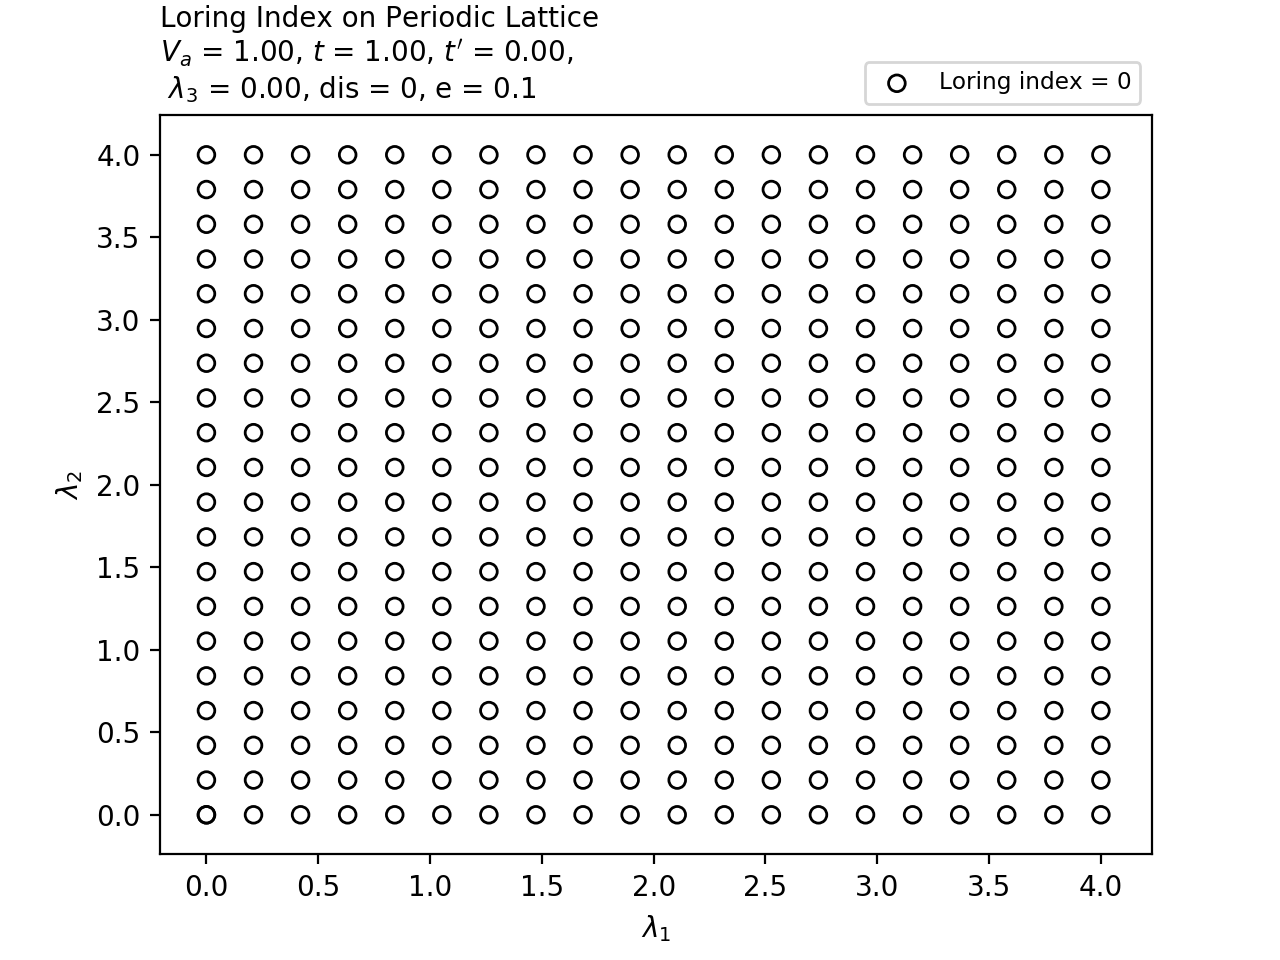
\includegraphics[width=.45\linewidth]{figures/periodic_triv} }}%
\subfloat{{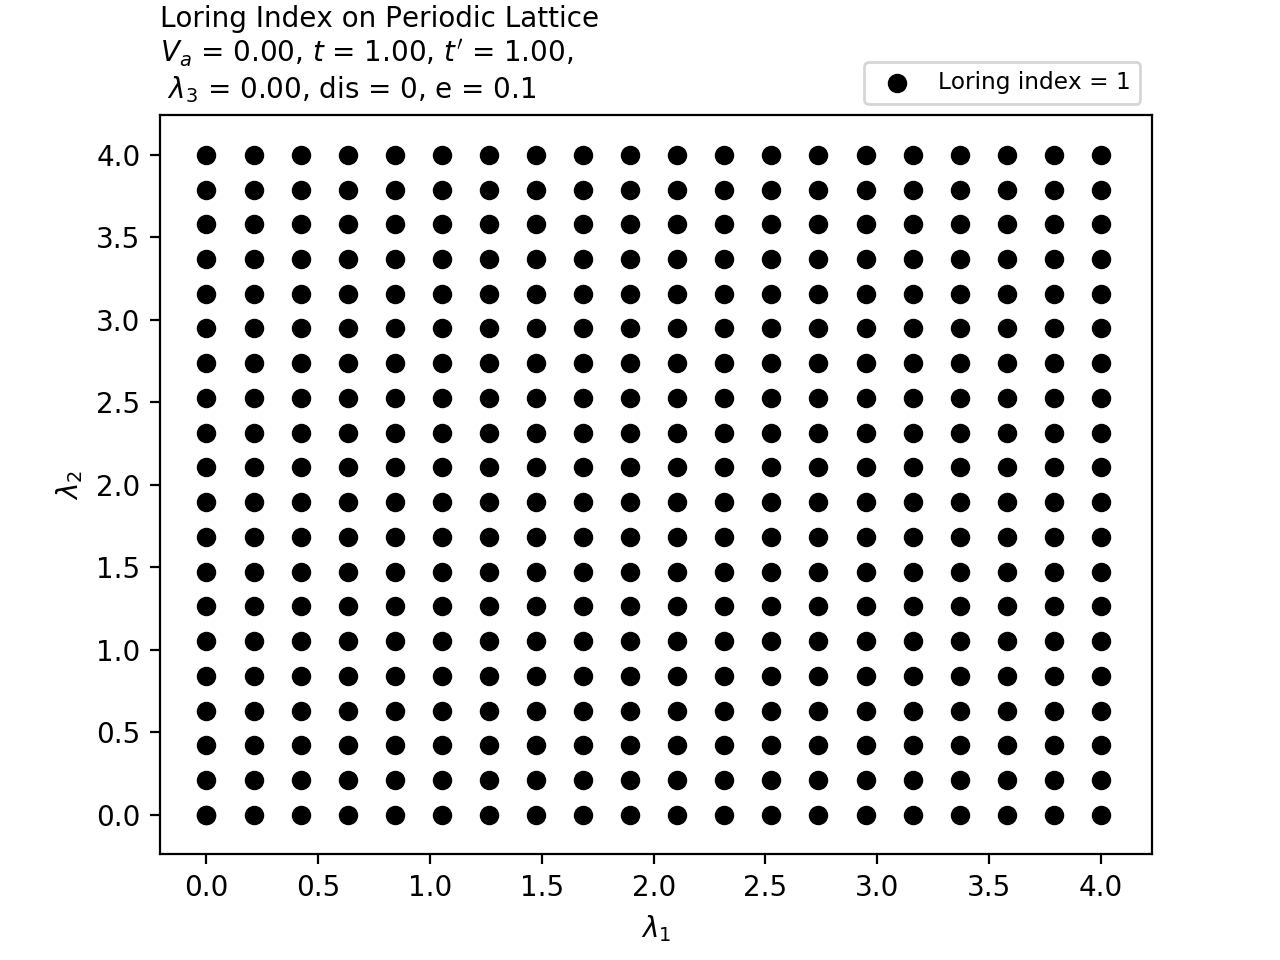
\includegraphics[width=.45\linewidth]{figures/periodic_top} }}%

\subfloat{{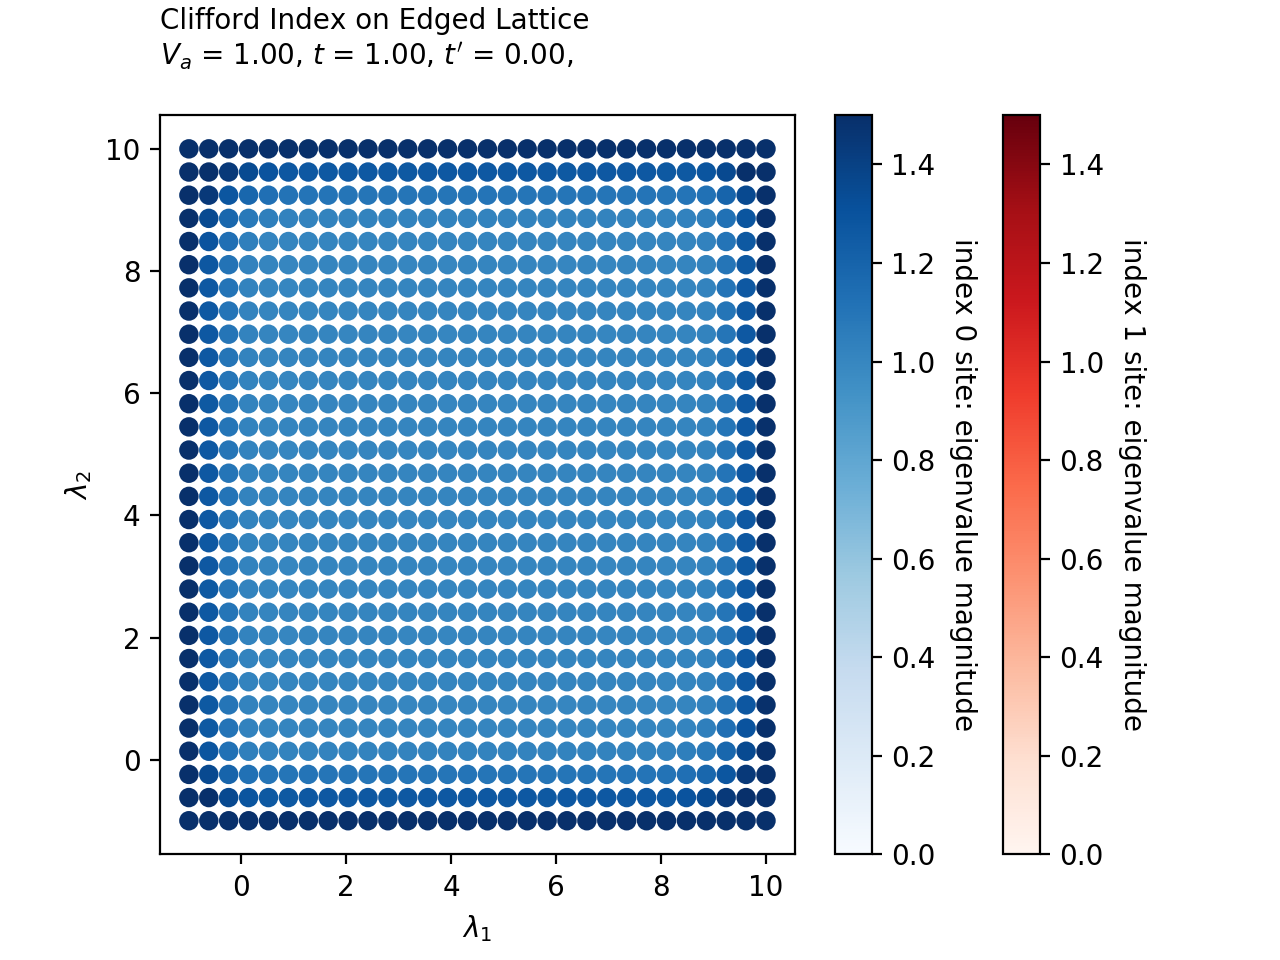
\includegraphics[width =.45\linewidth]{figures/edged_triv} }}%
\subfloat{{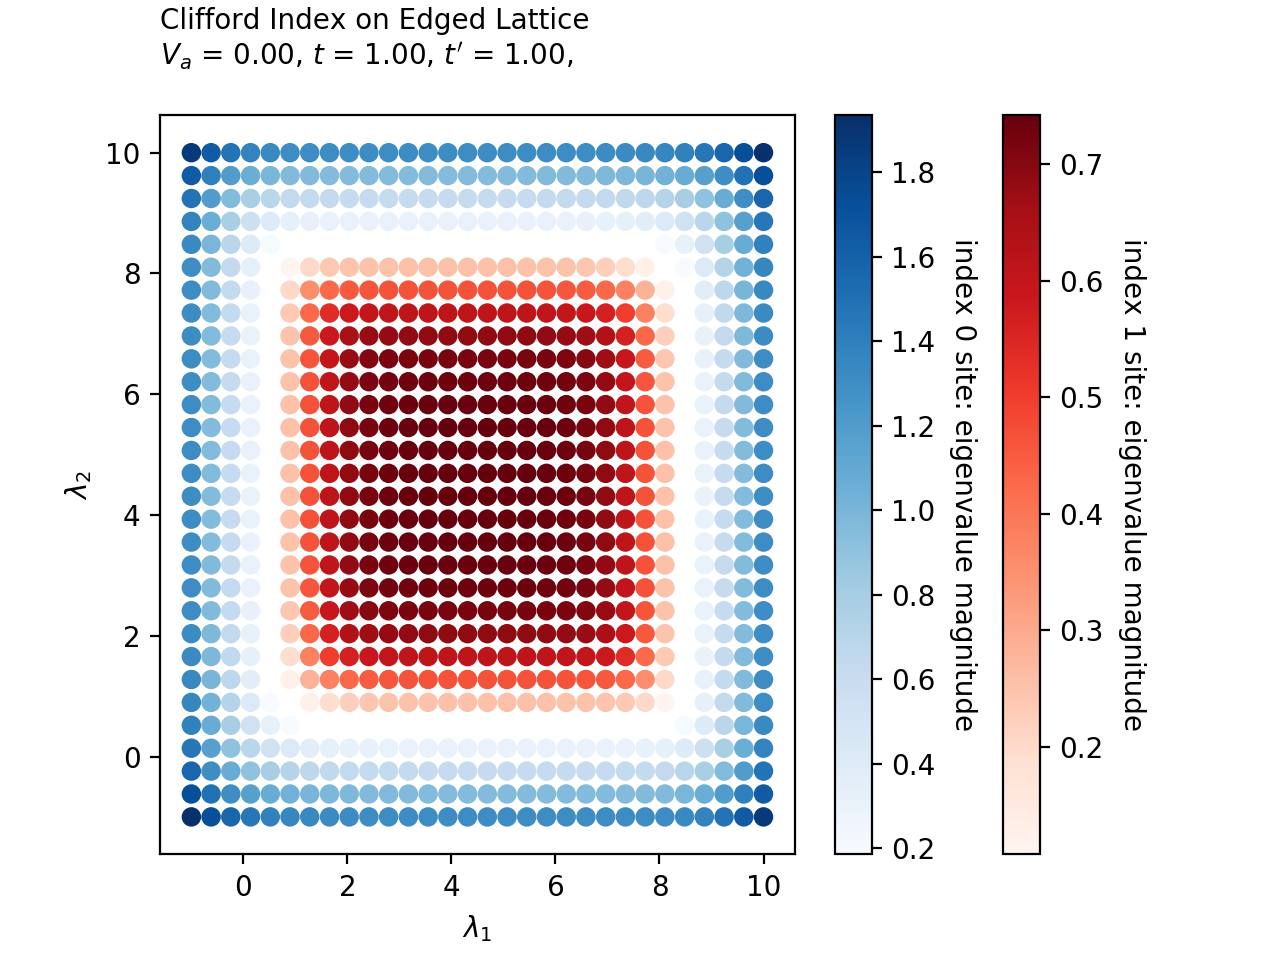
\includegraphics[width =.45\linewidth]{figures/edged_top} }}%
\caption{The top left is a trivial, periodic lattice; the top right is a topological, periodic lattice; the bottom left is a trivial, edged lattice; and the bottom right is a topological, edged lattice.
Each site in these figures represents a $(\lambda_1,\lambda_2,\lambda_3)$ triple with $\lambda_3 = 0$.
If a site is red, then it is in the pseudo-spectrum, i.e. $B(X - \lambda_1, Y - \lambda_2, H - \lambda_3)$ has a near-zero eigenvalue.
If a site is not in the pseudo-spectrum, then it is colored black for Bott index 1 and white for Bott index 0, where the Bott index is defined as one half the signature of $B$. \aw{very nice figure. It is a little funny that the corners for the Haldane model don't all look the same. I don't quite understand why this would be.} \jm{answer: Note that $B$ site on top right corner is only connected to one other site. Same for $A$ site on bottom left corner.}
\jm{update bottom right with new index plotting if time}
}%
\label{fig:haldane_index}%
\end{figure}
The advantage of the Clifford index compared to the Chern number is that the Chern number can only be defined on a periodic structure, whereas the Clifford index can be computed on non-periodic media.
We will use this advantage to study the robustness of waves on disorded media.

\section{Propagation in Haldane Model}
As expected, we find that localized states propagate along the boundary of the edged, topological lattice since this is a boundary between Bott index 0 and Bott index 1.

\begin{figure}
\centering
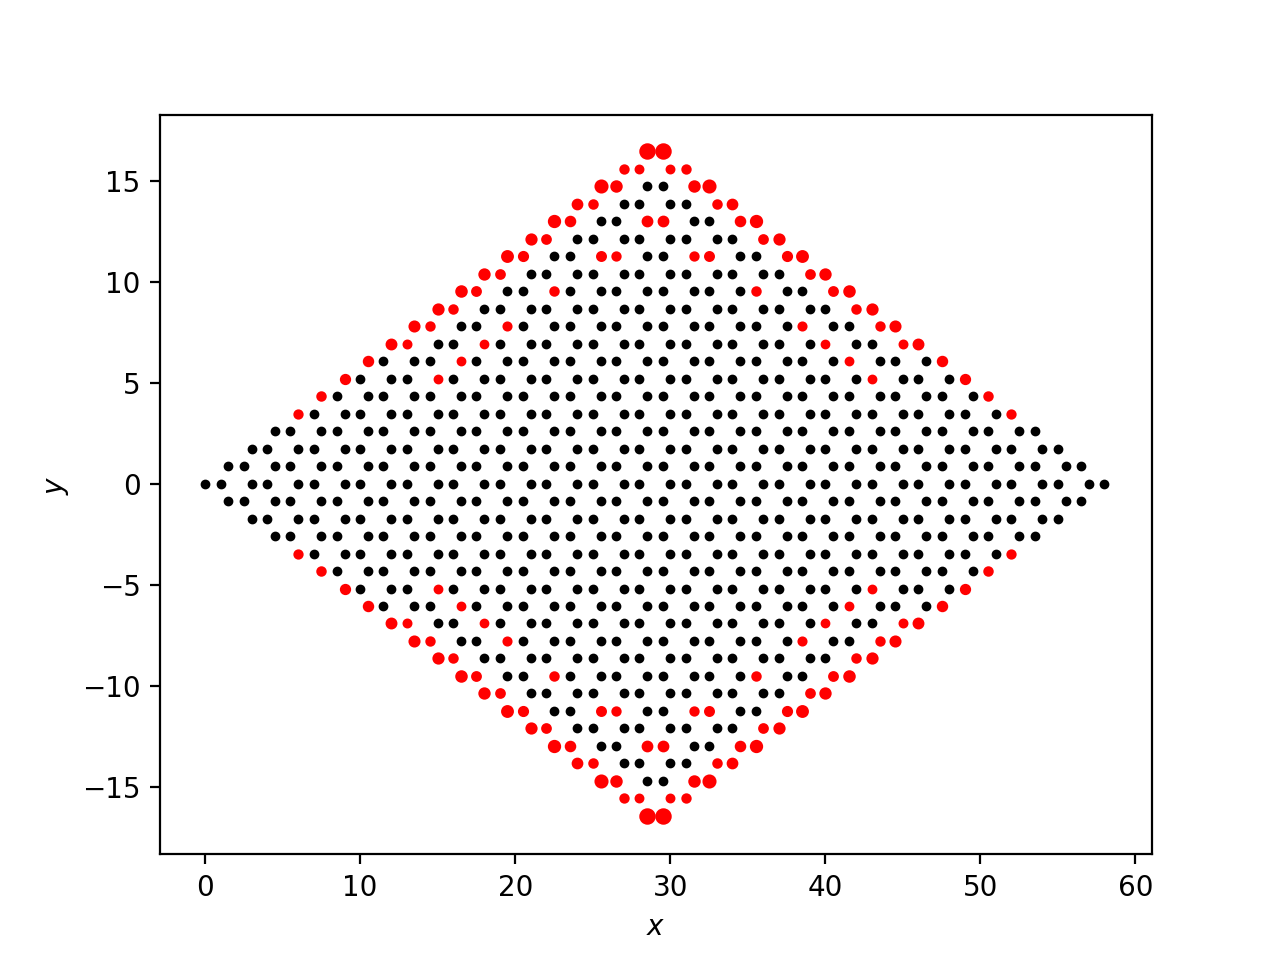
\includegraphics[width=.5\textwidth]{figures/haldane_estate.png}
\caption{Eigenstate of Haldane Model: this is the smallest magnitude eigenstate of the Hamiltonian of the Haldane hexagonal lattice.
The absolute value of an entry in the complex state vector, if larger than a specific threshold, is represented by the radius of a red circle.
Black circles only depict the lattice structure and are unrelated to the values of the eigenstate.
The sites have no onsite potential, but they do have neighbor and next-nearest neighbor hopping amplitudes: $V_a = V_b = 0,\; t = t' = 1$.
We see the state located on the edge of the lattice because this is a boundary between a region of Clifford index 0 and a region of Clifford index 1.
}
\label{fig:haldane_estate}%
\end{figure}

\begin{figure}
\centering
\subfloat{{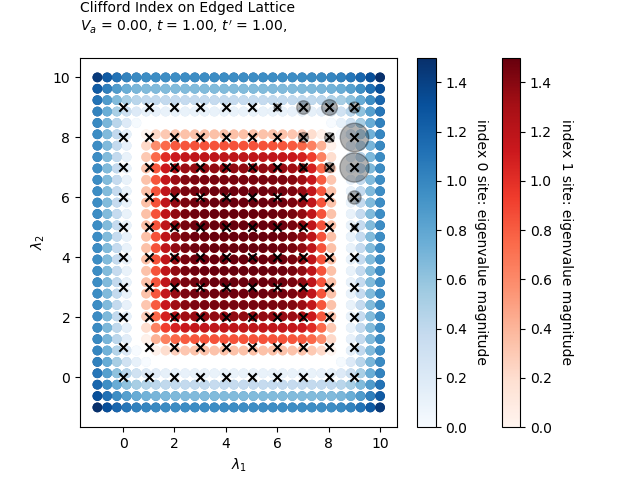
\includegraphics[width=.45\linewidth]{figures/haldane_propagation/img01.png} }}%
\subfloat{{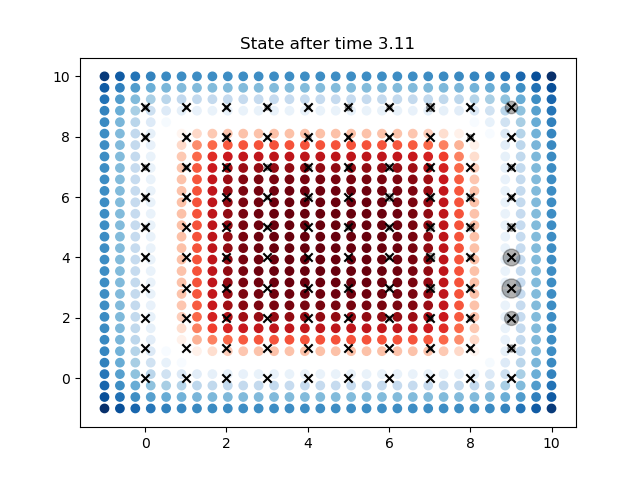
\includegraphics[width=.45\linewidth]{figures/haldane_propagation/img03.png} }}%

\subfloat{{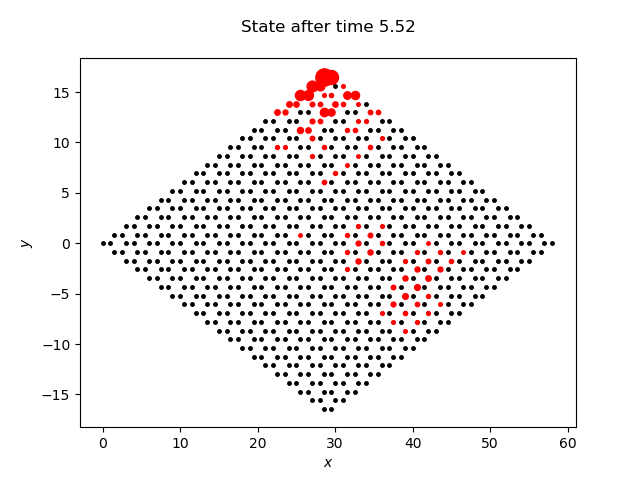
\includegraphics[width =.45\linewidth]{figures/haldane_propagation/img05.png} }}%
\subfloat{{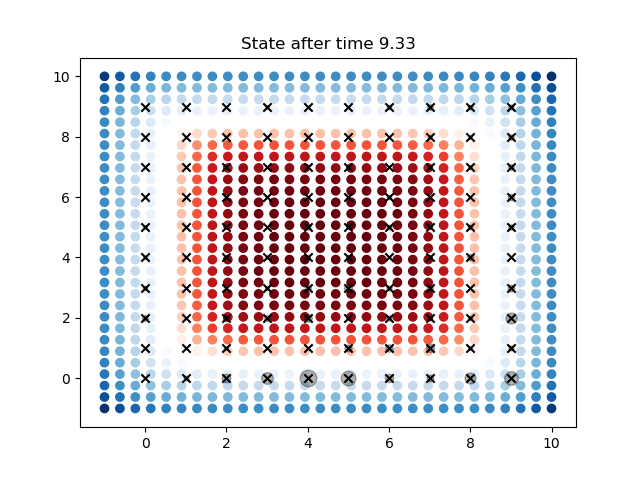
\includegraphics[width =.45\linewidth]{figures/haldane_propagation/img07.png} }}%

\subfloat{{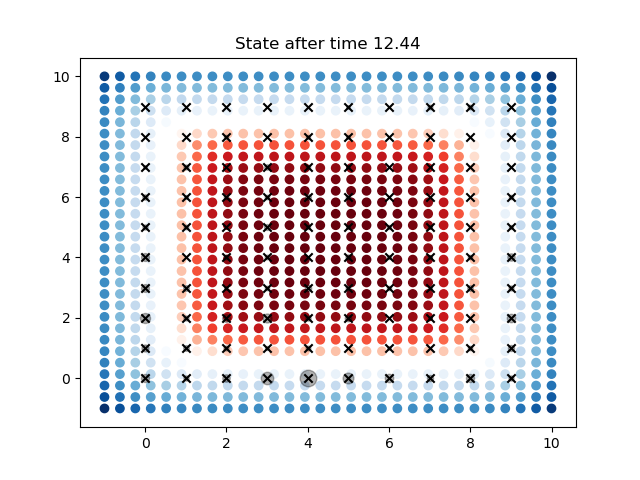
\includegraphics[width=.45\linewidth]{figures/haldane_propagation/img09.png} }}%
\subfloat{{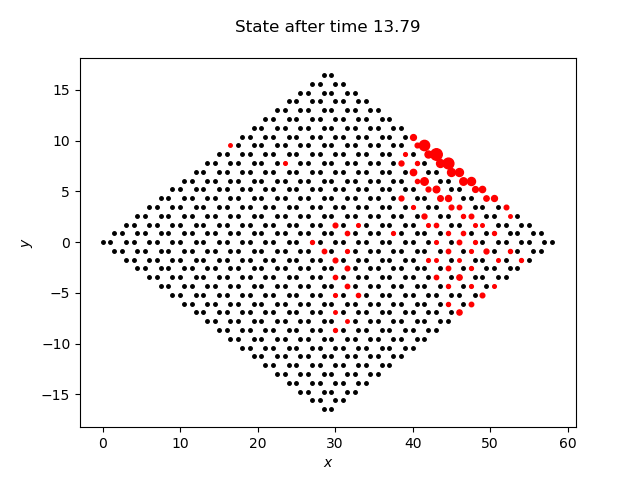
\includegraphics[width=.45\linewidth]{figures/haldane_propagation/img11.png} }}%

\subfloat{{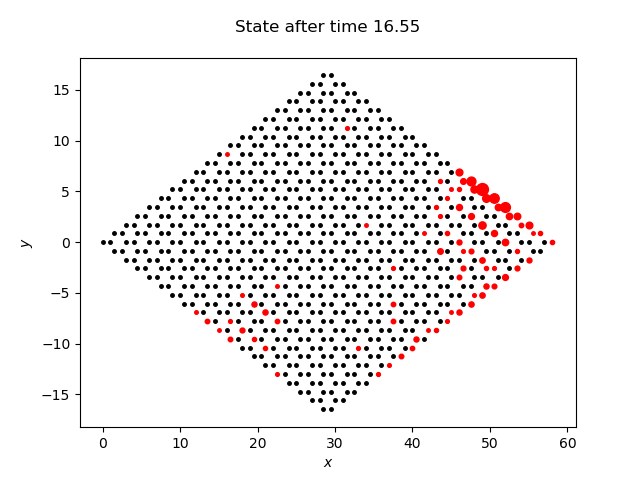
\includegraphics[width =.45\linewidth]{figures/haldane_propagation/img13.png} }}%
\subfloat{{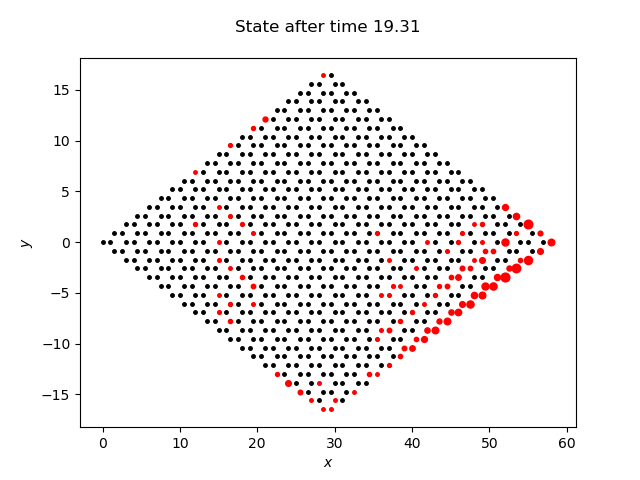
\includegraphics[width =.45\linewidth]{figures/haldane_propagation/img15.png} }}%
\caption{Propagation in Haldane Model: we localize the above eigenstate along one edge of the hexagonal lattice and simulate its propagation according to Schr{\"o}dinger's equation.
As before, the state is plotted in red and $V_a = V_b = 0,\; t = t' = 1$.
The state hits the corner and continues to propagate along the next edge, showing that it is unable to couple with bulk states.
}%
\label{fig:haldane_prop}%
\end{figure}

\aw{Clarify that this shows that the Bott index and Chern number predict edge states similarly}

\section{\texorpdfstring{$p_x + ip_y$}{px + ipy} Model}
\aw{We should mention why we work with a different model: the point is that it is unclear how to generalize the Haldane model to disordered media.}
Having shown that the Clifford index is equivalent to the Chern number as a topological index on periodic media which predicts the existence and robustness of edge states, we now see if the same holds true for disordered media, where the Chern number is not defined.
It is unclear how to generalize the Haldane model to disordered media, specifically because the hopping amplitudes when neighbors and next-nearest neighbors are no longer defined.
So we turn to a new model, the $p_x + ip_y$ model.
\jm{Is this why it is unclear?}

To construct this model, first generate a network of $N$ nodes (to be more consistent with physics we henceforth refer to nodes as sites) connected by edges. Define a Hilbert space $\mathcal{H}$ by associating to each site a copy of $\mathbb{C}^2$. The dimension of this space is clearly $2 N$. We denote vectors in $\mathcal{H}$ by:
\begin{equation}
	\psi = \left( \psi_1, \psi_2, ... \psi_N \right)^\top
\end{equation}
where each $\psi_j \in \mathbb{C}^2$:
\begin{equation}
	\psi_j = \left( \psi_j^A , \psi_j^B \right)^\top.
\end{equation}
We define a Hamiltonian acting on the $j$th site of the network by:
\begin{equation}
	( H \psi )_j = H_{jj} \psi_j + \sum_{ k \text{ nearest neighbors of } j } H_{jk} \psi_k,
\end{equation}
where $H_{jj}$ and $H_{jk}$ are $2 \times 2$ matrices defined by:
\begin{equation}
	H_{jj} = - \mu \sigma_z,
\end{equation}
\begin{equation}
	H_{jk} = - t \sigma_z - \frac{ i }{ 2 } \Delta \sigma_x \cos( \alpha_{jk} ) - \frac{ i }{ 2 } \Delta \sigma_y \sin( \alpha_{jk} ).
\end{equation}
Here, $\mu, t, \Delta$ are real parameters,
\begin{equation}
	\sigma_x = \begin{pmatrix} 0 & 1 \\ 1 & 0 \end{pmatrix}, \quad \sigma_y = \begin{pmatrix} 0 & - i \\ i & 0 \end{pmatrix}, \quad \sigma_z = \begin{pmatrix} 1 & 0 \\ 0 & -1 \end{pmatrix},
\end{equation}
denote the Pauli matrices, and $\alpha_{jk}$ denotes the angle of the edge between the $j$ and $k$th site relative to the $x$ axis (see second slide of \verb|Loring_slides.pdf| in \verb|related_papers| directory).

Compared with the Haldane model, $\mu$ plays the role of $V^A$ (onsite potential difference between $A$ and $B$ sites, assuming $V^B = - V^A$), $t$ plays the role of $t$ (real nearest neighbor hopping), and $\Delta$ plays the role of $t'$ (strength of complex hopping). The nice thing about this model is that it involves only nearest neighbor hopping, so it is relatively easy to generalize to structures without periodicity.

In the case of a perfect square lattice the model simplifies to the following: 
\begin{equation}
\begin{split}
	(H \psi)_{mn} &= - \mu \sigma_z \psi_{mn} - t \sigma_z \left( \psi_{m+1,n} + \psi_{m-1,n} + \psi_{m,n+1} + \psi_{m,n-1} \right) \\
	&+ \frac{ i \Delta }{ 2 } \left( - \sigma_x \psi_{m+1,n} - \sigma_y \psi_{m,n+1} + \sigma_x \psi_{m-1,n} + \sigma_y \psi_{m,n-1} \right),
\end{split}
\end{equation}
where $m$ denotes the co-ordinate in the $x$ direction and $n$ denotes that in the $y$ direction. Imposing the Bloch-periodic boundary condition yields:
\begin{equation}
\begin{split}
	H(k) \psi &= \left[ - \mu \sigma_z - t \left( e^{i k_1} + e^{- i k_1} + e^{i k_2} + e^{- i k_2} \right) \sigma_z \right. \\
	&\left. + \frac{ i \Delta }{ 2 } \left( -  e^{i k_1} + e^{- i k_1} \right) \sigma_x + \frac{ i \Delta }{ 2 } \left( - e^{i k_2} + e^{- i k_2} \right) \sigma_y \right] \psi,
\end{split}
\end{equation}
\begin{equation}
	H(k) \psi = \left[ - \mu \sigma_z - 2 t \left( \cos(k_1) + \cos(k_2) \right) \sigma_z + \Delta \sin(k_1) \sigma_x + \Delta \sin(k_2) \sigma_y \right] \psi. 
\end{equation}
So:
\begin{equation}
	H(k) = \begin{pmatrix} - \mu - 2 t ( \cos k_1 + \cos k_2 ) & \Delta ( \sin k_1 - i \sin k_2 ) \\ \Delta ( \sin k_1 + i \sin k_2 ) & \mu + 2 t ( \cos k_1 + \cos k_2 ) \end{pmatrix}.
\end{equation}
Eigenvalues $E$ satisfy the characteristic equation:
\begin{equation}
	( - \mu - 2 t ( \cos k_1 + \cos k_2 ) - E )( \mu + 2 t ( \cos k_1 + \cos k_2 ) - E ) - \Delta^2 ( \sin^2 k_1 + \sin^2 k_2 ) = 0
\end{equation}
which has the solution:
\begin{equation}
	E = \pm 2 t \sqrt{ (\Delta')^2 \sin^2 k_1 + (\Delta')^2 \sin^2 k_2 + \left( \mu' + \cos k_1 + \cos k_2 \right)^2 },
\end{equation}
where:
\begin{equation}
	\Delta' := \frac{\Delta}{2 t} \quad \mu' := \frac{ \mu }{ 2 t }
\end{equation}
and now under the square root is a sum of non-negative terms. For the bands to touch (i.e. for what is under the spectral gap to vanish) it must be that:
\begin{equation}
	k_1 = m \pi \quad k_2 = n \pi
\end{equation}
for $m \in \{0,1\}$ and $n \in \{0,1\}$, and:
\begin{equation}
	\mu' + \cos m \pi + \cos n \pi = 0.
\end{equation}
This can only occur if $m = n = 1$ and $\mu' = 2$, if $m \neq n$ and $\mu' = 0$, or if $m = n = 0$ and $\mu' = - 2$. These are the only values of $\mu'$ such that a topological transition (a change in the Chern number) can happen. \aw{it would be nice to check this numerically. We should be able to use the code we wrote in the summer to compute the Chern number of the Haldane model. I believe that the Chern number is 1 for $0 \leq \mu' \leq 2$, -1 for $- 2 \leq \mu' \leq 0$, and 0 otherwise. But we should check this.}

\section{Loring Index in \texorpdfstring{$p_x + ip_y$}{px + ipy} Model}
\jm{what should we call this model?}
For the \texorpdfstring{$p_x + ip_y$}{px + ipy} model we compute X and Y as before in the Haldane model. Nodes in the \texorpdfstring{$p_x + ip_y$}{px + ipy} model consist of two sites (labeled A and B) just as in the Haldane model the X and Y matrices represent this in that they are diagonal matrices of size 2*m*m. We also compute pseudo-spectrum and Bott index as before, and get a similar result of a topological case which exhibits a transition from Bott index 0 at the edge to +1 on the interior. Again, this is a situation in which the system is general and not periodic so the Bott index is useful, as we cannot use the Chern number. The fact that we see very similar behavior in this model is very significant and supports the idea that the Bott index is a general invariant than can be calculated regardless of periodicity or structure.

\begin{figure}
\centering
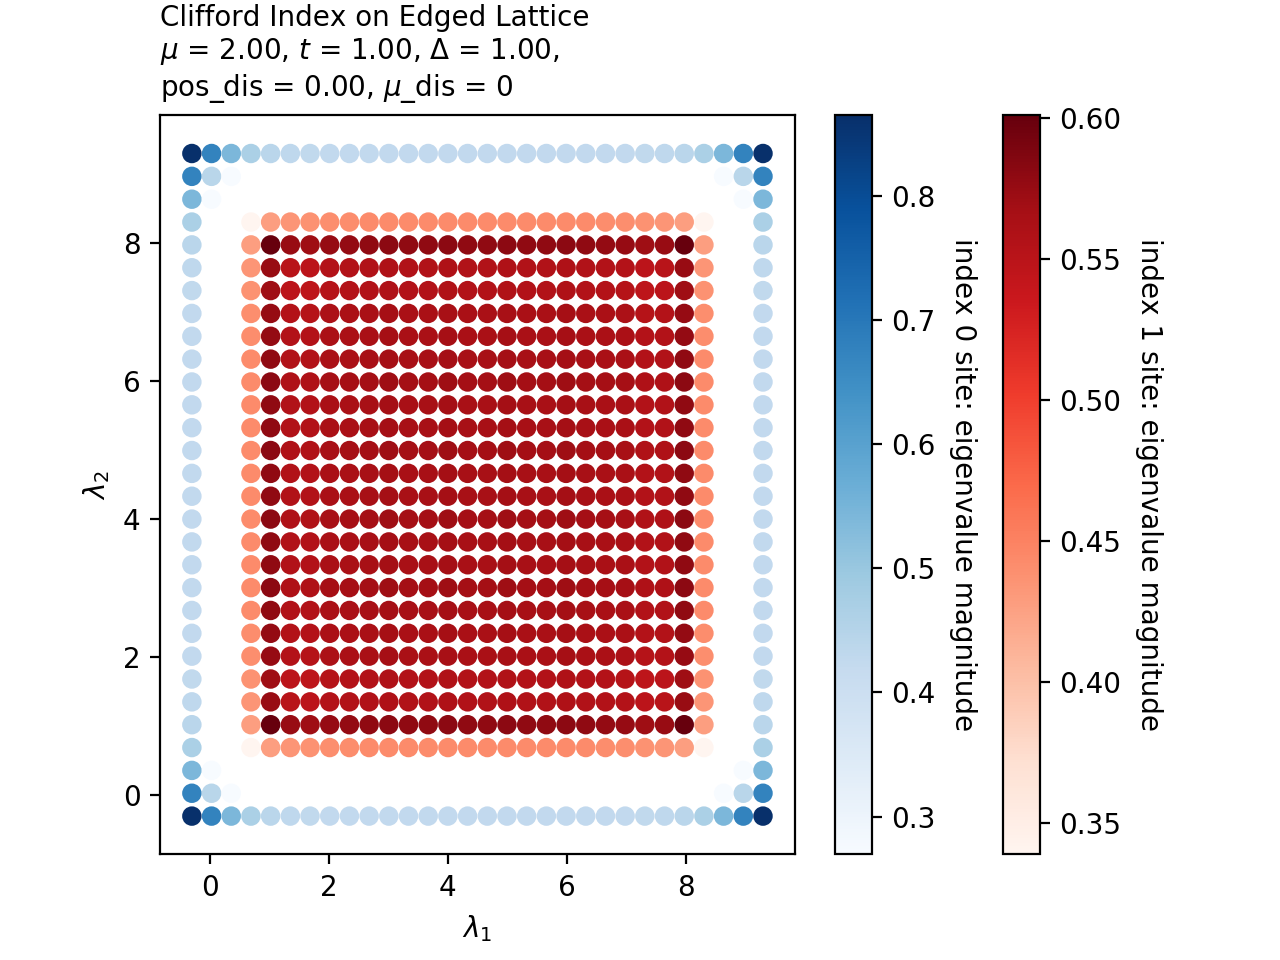
\includegraphics[width=.9\textwidth]{figures/pxipy_clifford.png}
\caption{Clifford Index in $p_x + ip_y$ Model: plotted here is the Clifford pseudospectrum.
The sites which are colored red and blue represent sites in the pseudospectrum.
A site with $x$-coordinate $\lambda_1$ and $y$-coordinate $\lambda_2$ is in the pseudospectrum if the matrix $B(X - \lambda_1, Y - \lambda_2, H - \lambda_3)$ \eqref{eq:B_matrix} has an eigenvalue with absolute value smaller than a given threshold, in this case $0.25$.
If a site is not in the psuedospectrum, we calculate its index using \eqref{eq:index}.
(Note that even thought the color bar on the right is only valued on $[-0.17,0.17]$, the threshold for pseudospectrum is still $0.25$.)
}
\label{fig:pxipy_index}%
\end{figure}

\begin{figure}
\centering
\subfloat{{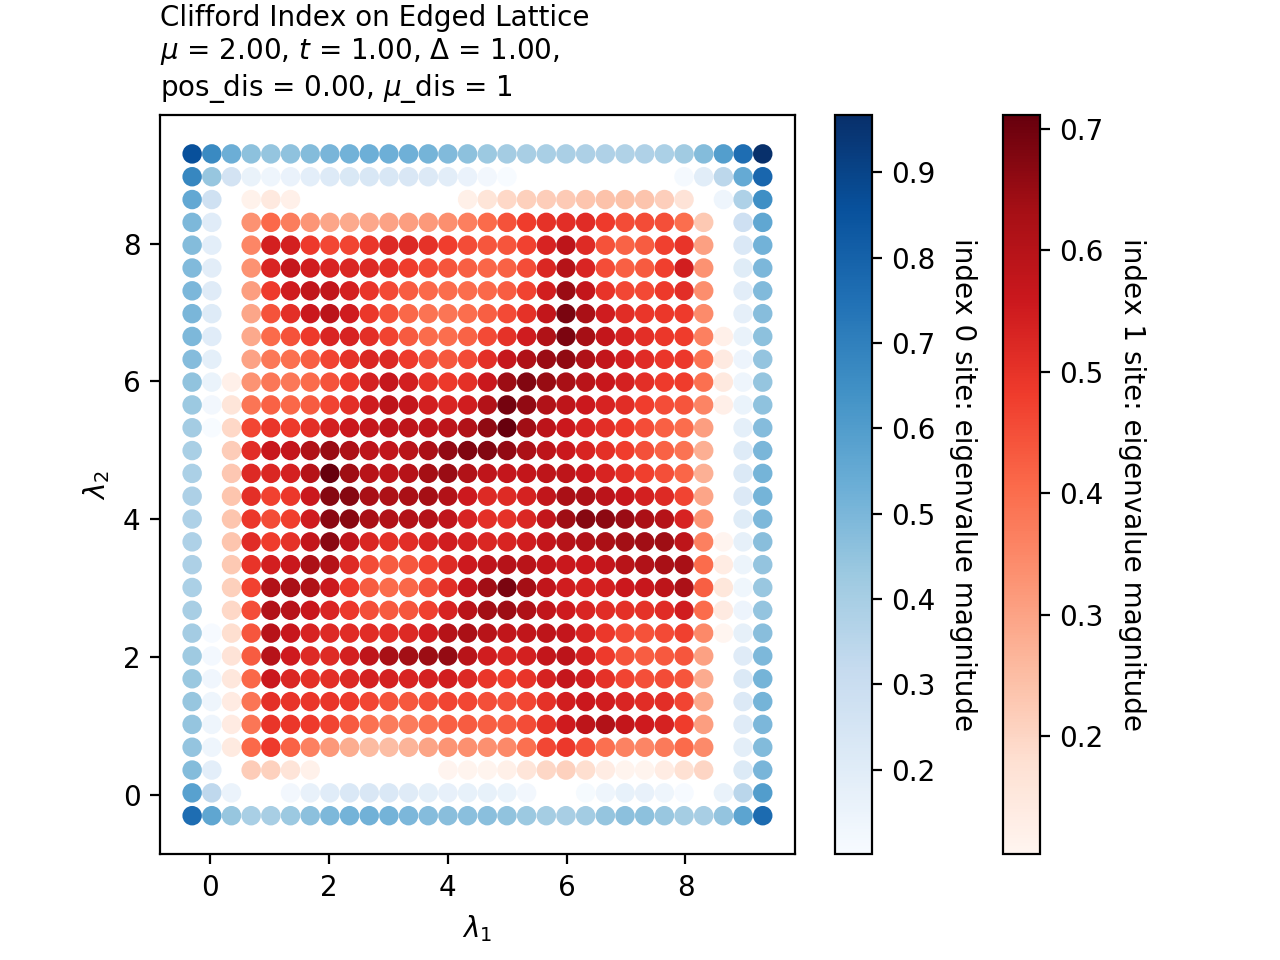
\includegraphics[width=.45\linewidth]{figures/mu_dis_index/img01.png} }}%
\subfloat{{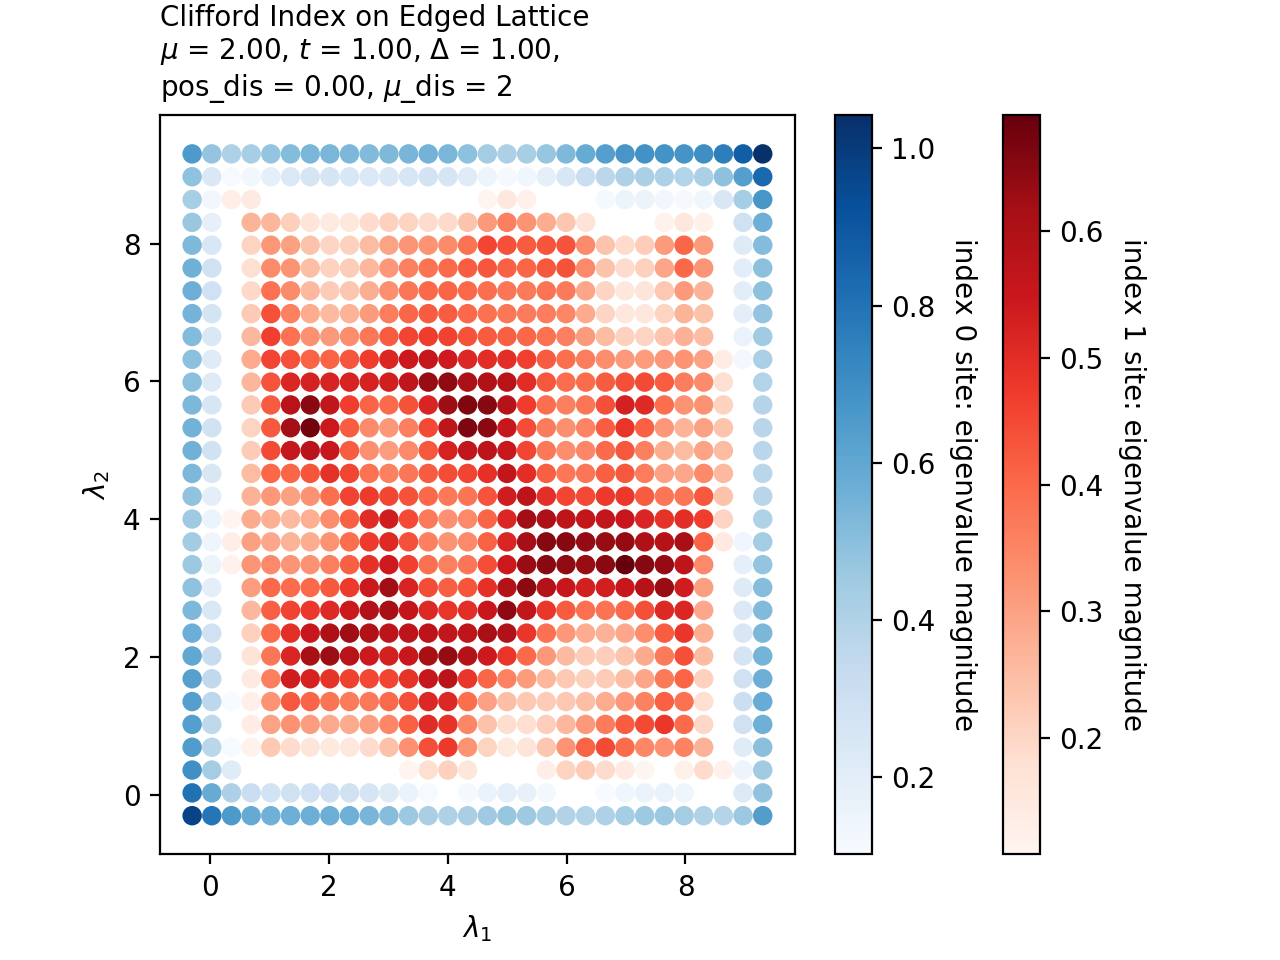
\includegraphics[width=.45\linewidth]{figures/mu_dis_index/img02.png} }}%

\subfloat{{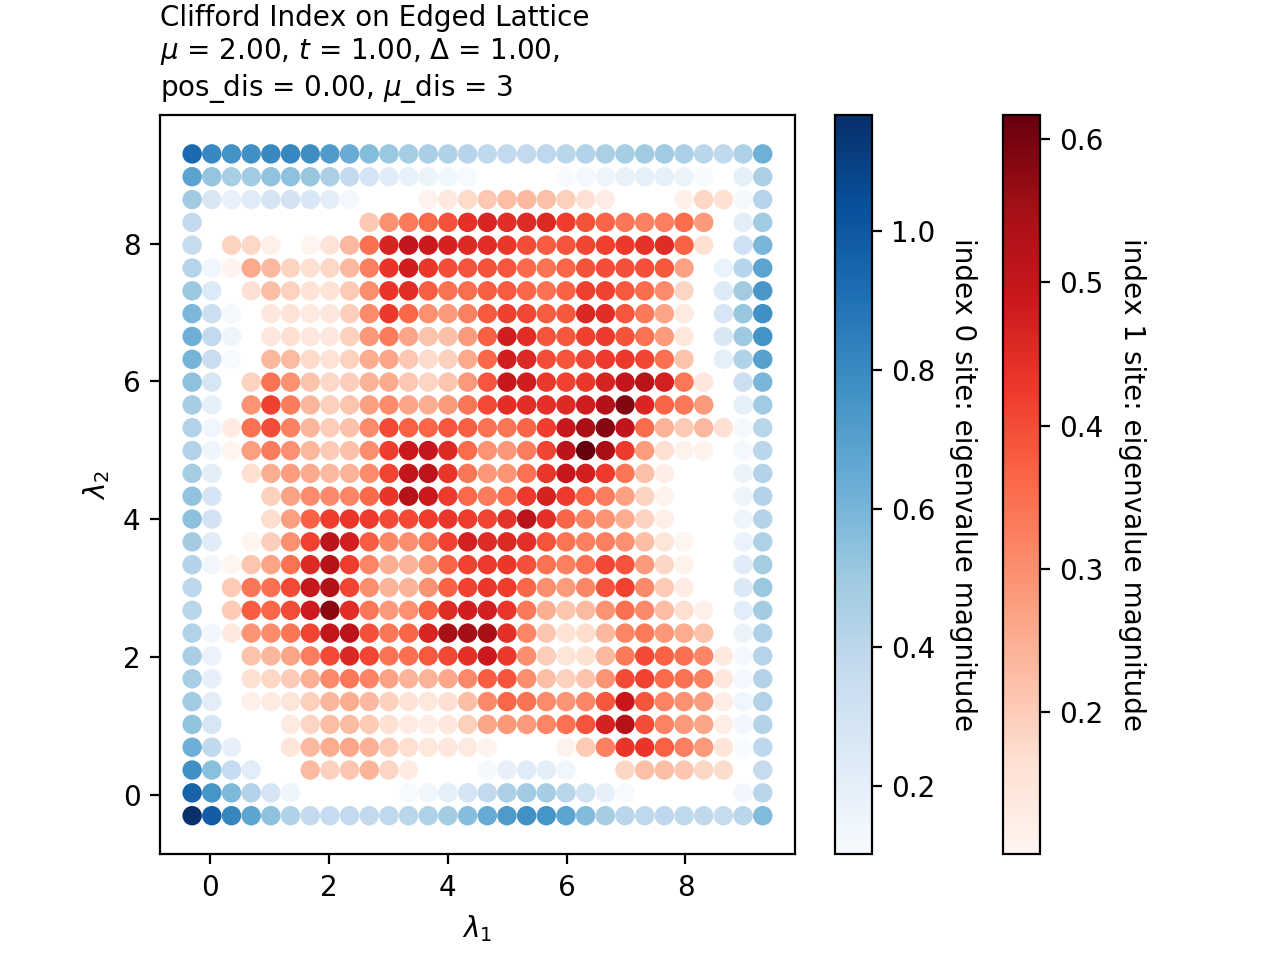
\includegraphics[width =.45\linewidth]{figures/mu_dis_index/img03.png} }}%
\subfloat{{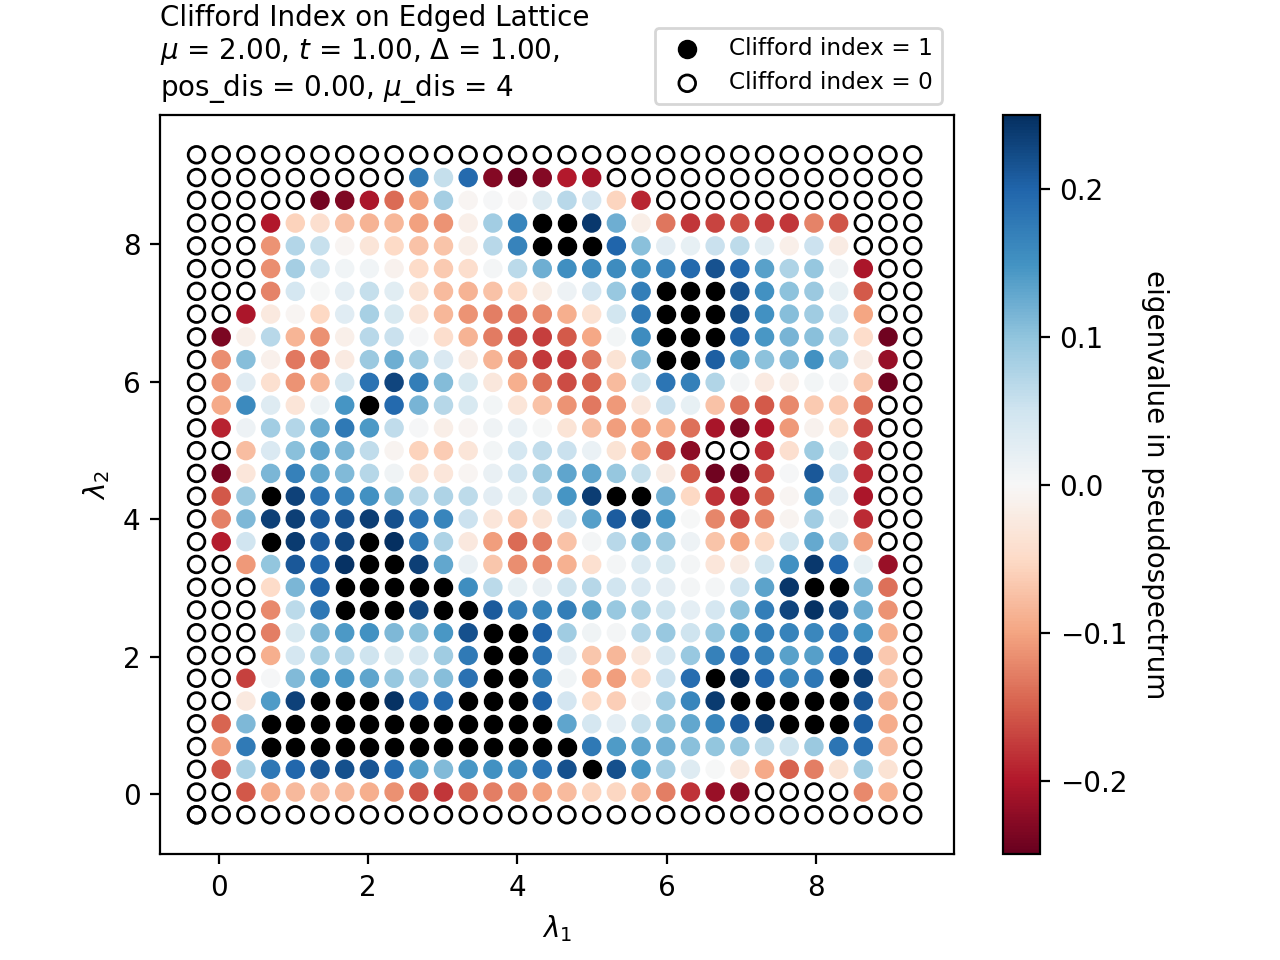
\includegraphics[width =.45\linewidth]{figures/mu_dis_index/img04.png} }}%

\caption{Clifford Index in $p_x + ip_y$ Model with Onsite Disorder: we plot the pseudospectrum and index of lattice sites with varying degrees of onsite disorder.
The potential energy of each site on the lattice is chosen randomly from a uniform distribution centered at $\mu$ with the length of the interval equal to a disorder parameter: 1, 2, 3, and 4 in these plots.
So going from left to right, top to bottom, $\mu$ was chosen uniformly on $[1.5,2.5],\; [1,3],\;[0.5,3.5],$ and $[0,4]$, respectively.
Again, blue and red represents sites in the pseudospectrum, and black indicates index 1, while white circles indicate index 0.
}%
\label{fig:mu_dis_index}%
\end{figure}

\section{Propagation in \texorpdfstring{$p_x + ip_y$}{px + ipy} Model}

\begin{figure}
\centering
\subfloat{{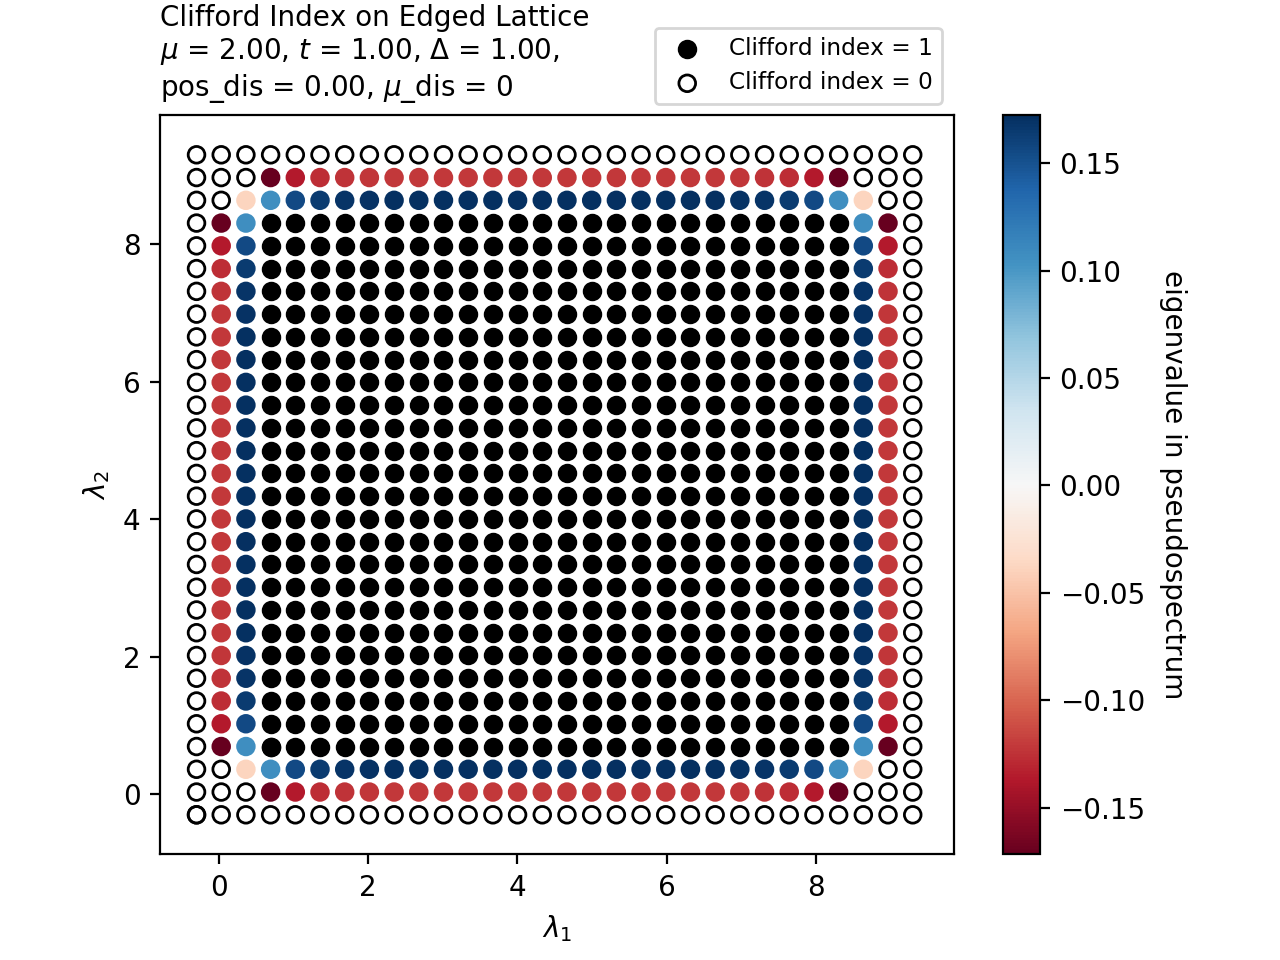
\includegraphics[width=.45\linewidth]{figures/pxipy_prop/index.png} }}%
\subfloat{{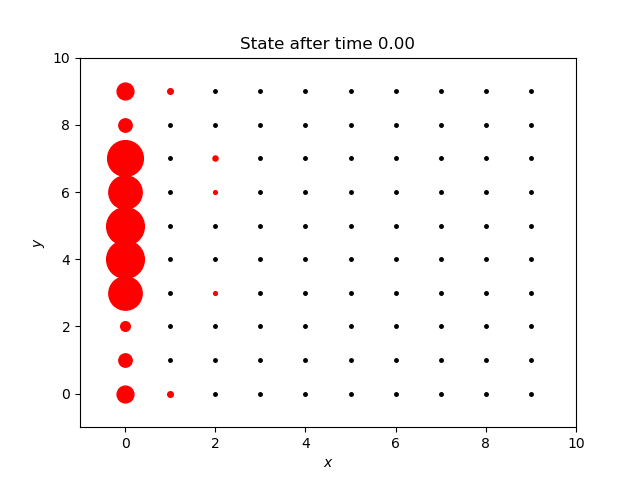
\includegraphics[width=.45\linewidth]{figures/pxipy_prop/img01.png} }}%

\subfloat{{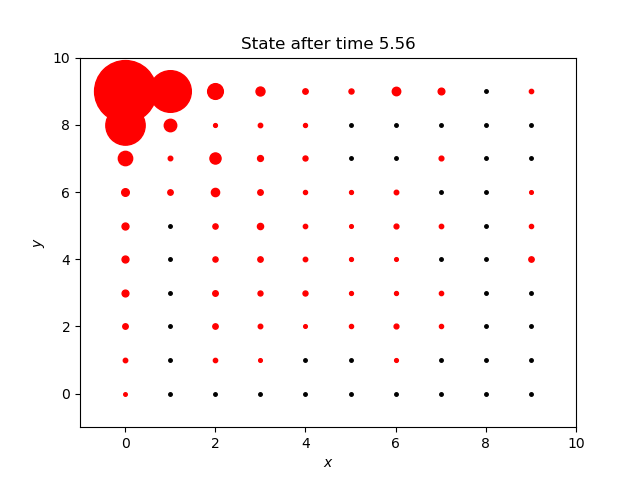
\includegraphics[width =.45\linewidth]{figures/pxipy_prop/img02.png} }}%
\subfloat{{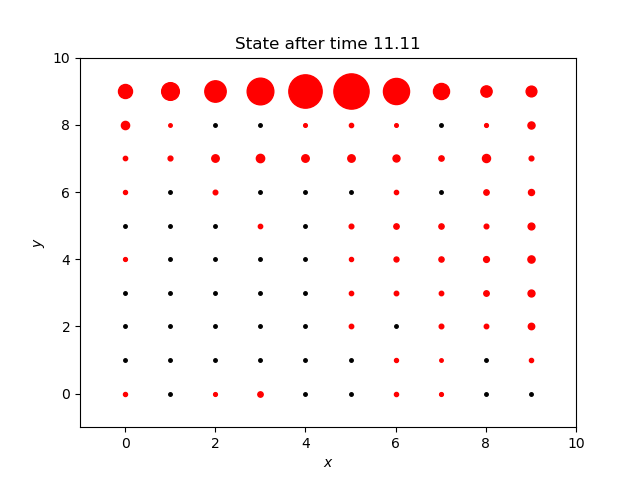
\includegraphics[width =.45\linewidth]{figures/pxipy_prop/img03.png} }}%

\subfloat{{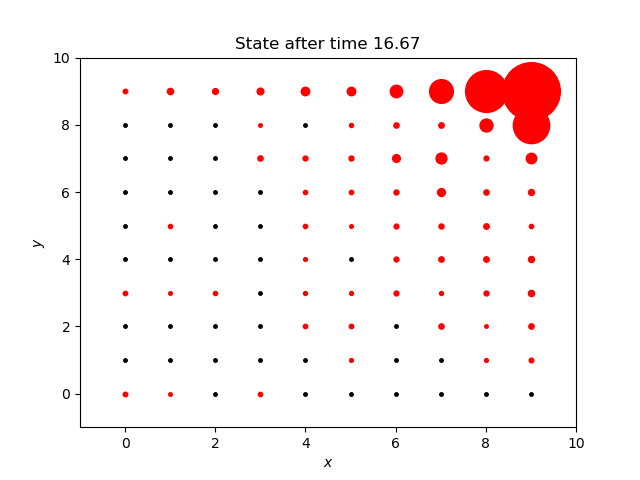
\includegraphics[width=.45\linewidth]{figures/pxipy_prop/img04.png} }}%
\subfloat{{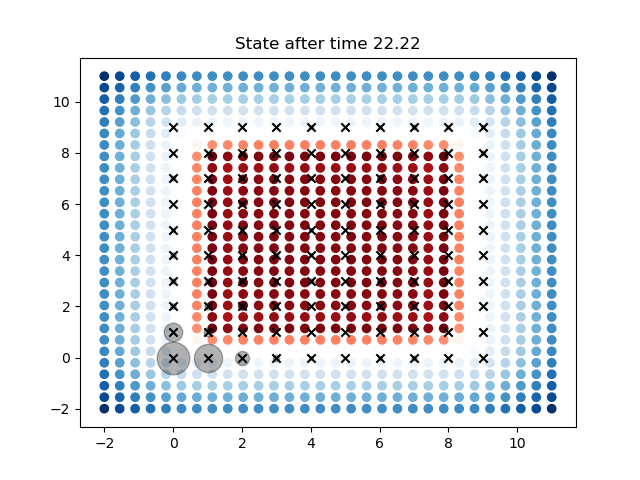
\includegraphics[width=.45\linewidth]{figures/pxipy_prop/img05.png} }}%

\subfloat{{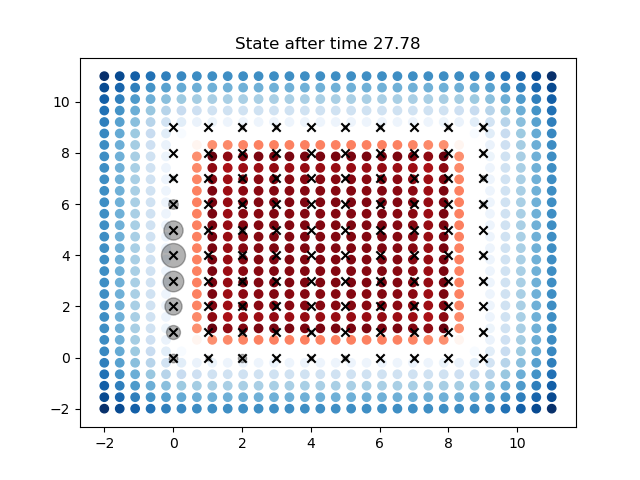
\includegraphics[width =.45\linewidth]{figures/pxipy_prop/img06.png} }}%
\subfloat{{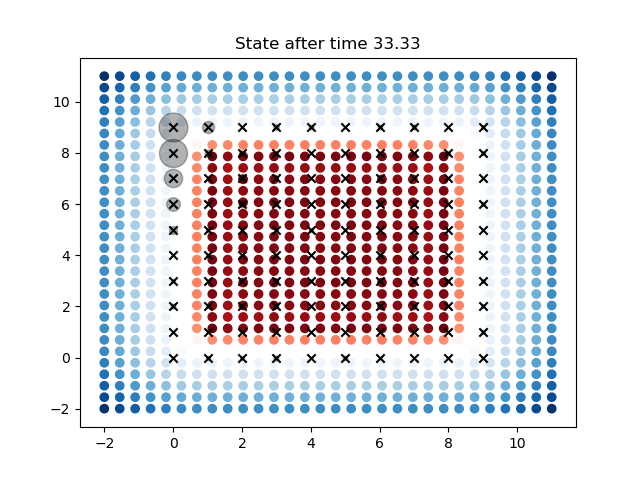
\includegraphics[width =.45\linewidth]{figures/pxipy_prop/img07.png} }}%
\caption{Propagation in $p_x + ip_y$ Model: we localize the above eigenstate along one edge of the lattice and simulate its propagation according to Schr{\"o}dinger's equation.
As before, the state is plotted in red and $\mu = 2,\; t = \Delta = 1$.
The state propagates along the edge.
}%
\label{fig:pxipy_prop}%
\end{figure}

\begin{figure}
\centering
\subfloat{{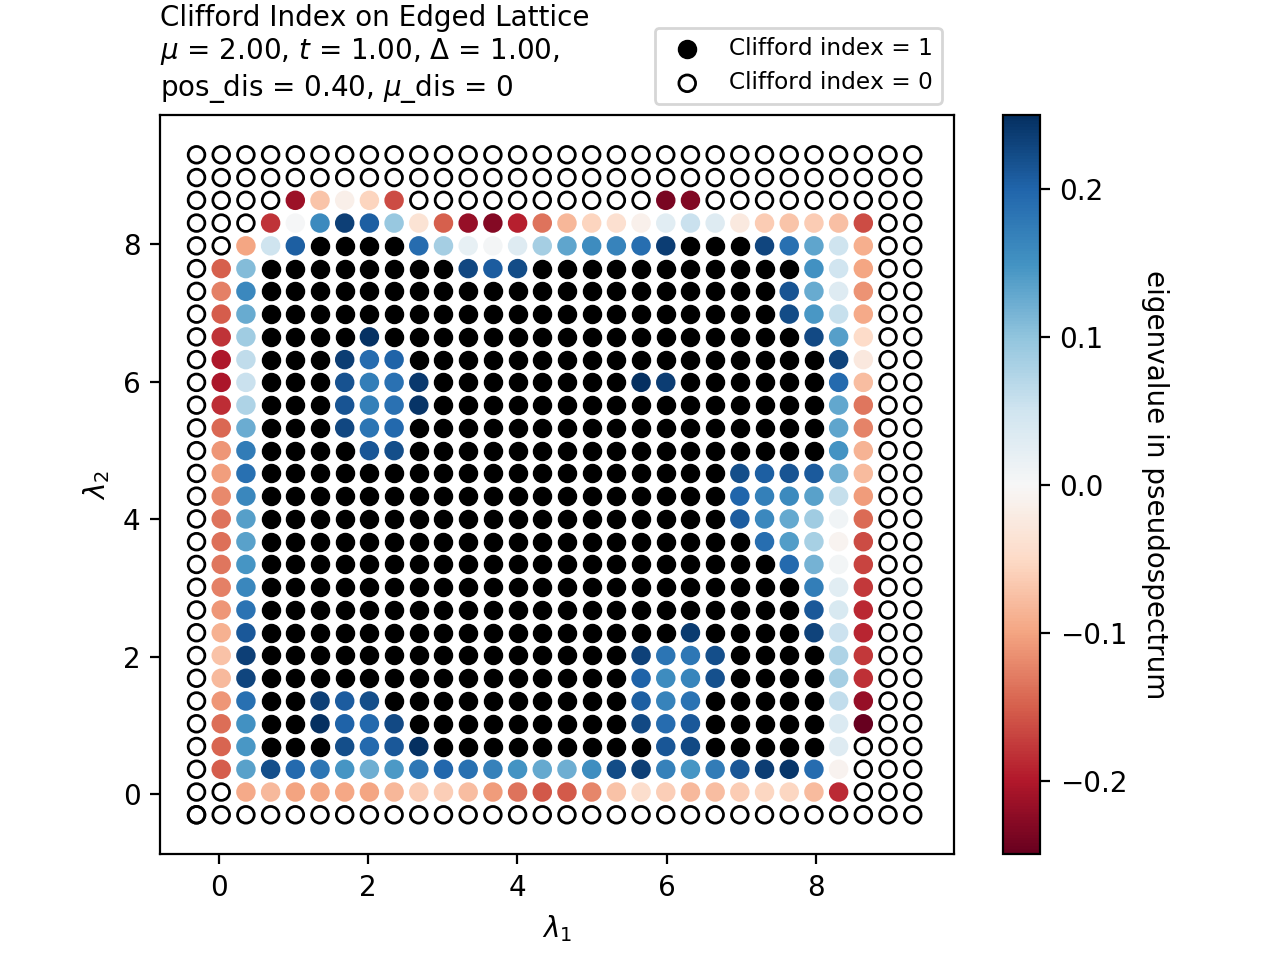
\includegraphics[width=.45\linewidth]{figures/pxipy_posdis/index.png} }}%
\subfloat{{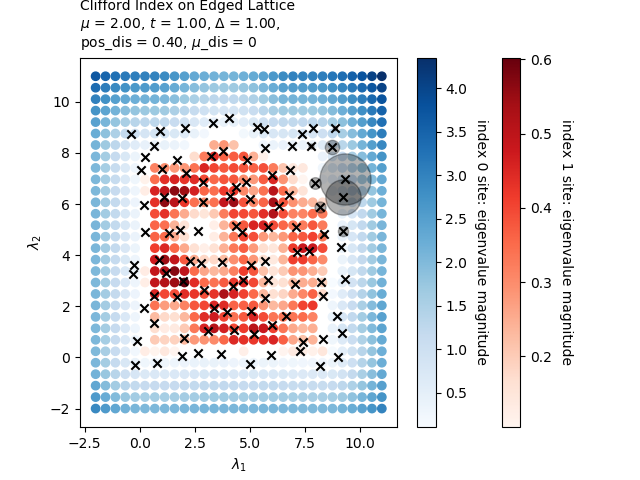
\includegraphics[width=.45\linewidth]{figures/pxipy_posdis/img01.png} }}%

\subfloat{{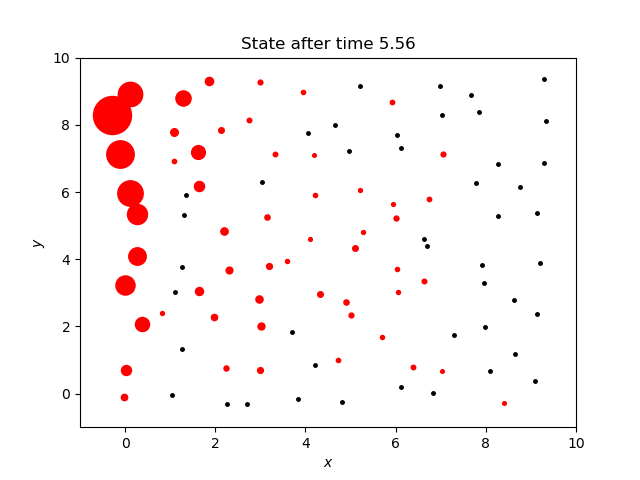
\includegraphics[width =.45\linewidth]{figures/pxipy_posdis/img02.png} }}%
\subfloat{{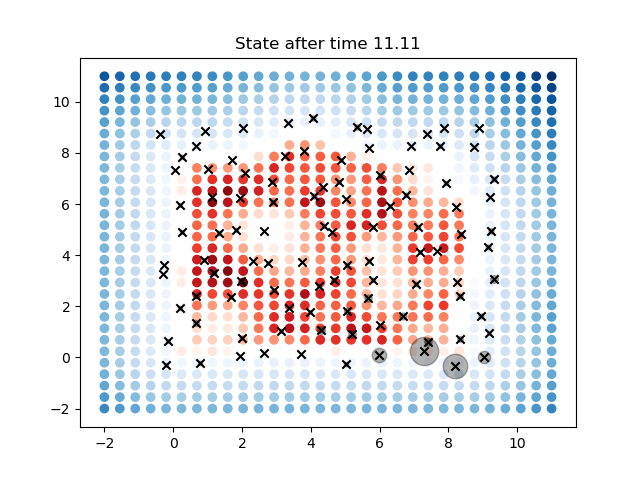
\includegraphics[width =.45\linewidth]{figures/pxipy_posdis/img03.png} }}%

\subfloat{{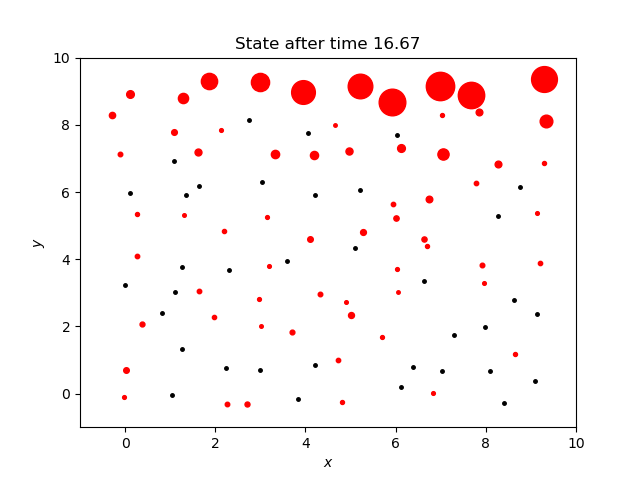
\includegraphics[width=.45\linewidth]{figures/pxipy_posdis/img04.png} }}%
\subfloat{{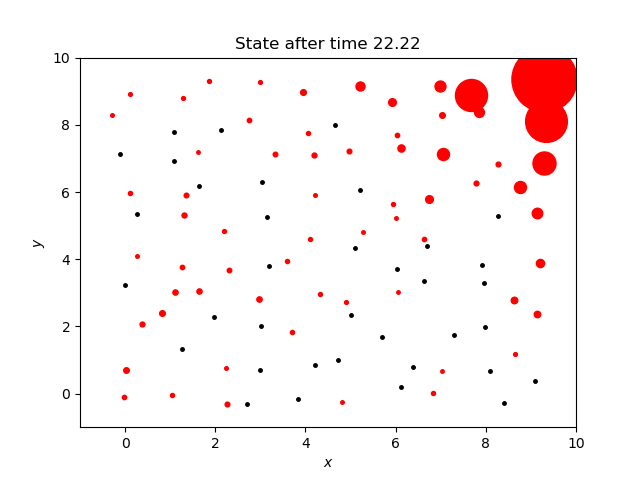
\includegraphics[width=.45\linewidth]{figures/pxipy_posdis/img05.png} }}%

\subfloat{{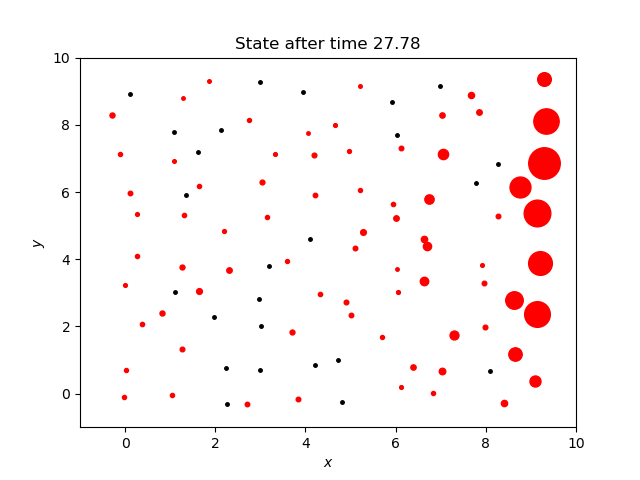
\includegraphics[width =.45\linewidth]{figures/pxipy_posdis/img06.png} }}%
\subfloat{{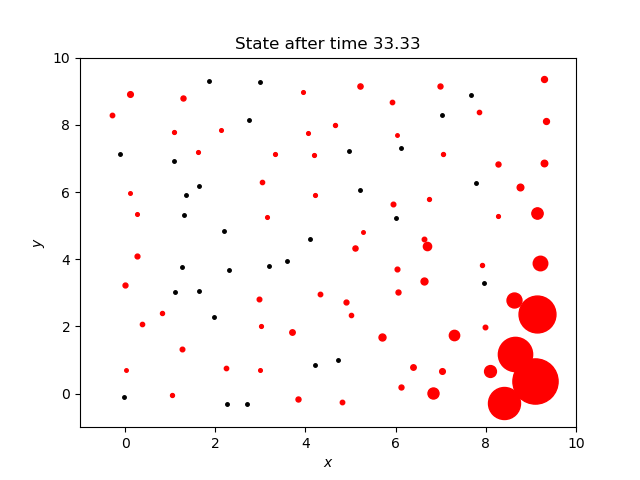
\includegraphics[width =.45\linewidth]{figures/pxipy_posdis/img07.png} }}%
\caption{Propagation in $p_x + ip_y$ Model with Position Disorder: with parameters as in Figure \ref{fig:pxipy_prop}, we now add position disorder to the lattice, i.e. we let the $x$ and $y$ coordinates of each site vary uniformly on an interval centered at its original coordinate in the lattice.
In this case, sites can deviate up to $0.4$ from its original position in either the $x$ or $y$ direction.
We see continued propagation around the edge as in the case with no disorder.
}%
\label{fig:pos_dis_prop}%
\end{figure}

\begin{figure}
\centering
\subfloat{{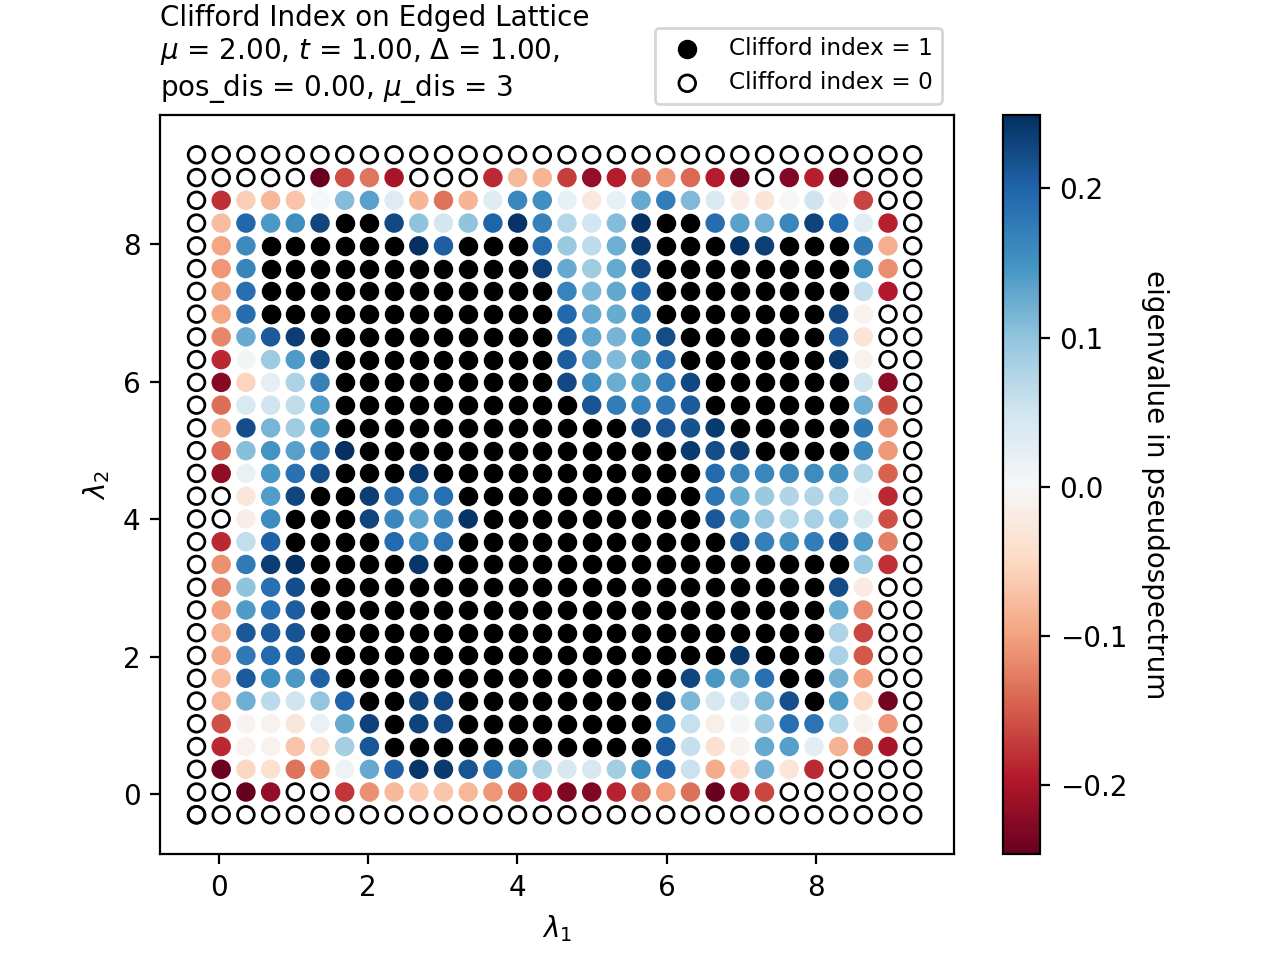
\includegraphics[width=.45\linewidth]{figures/mu_dis_edge/index.png} }}%
\subfloat{{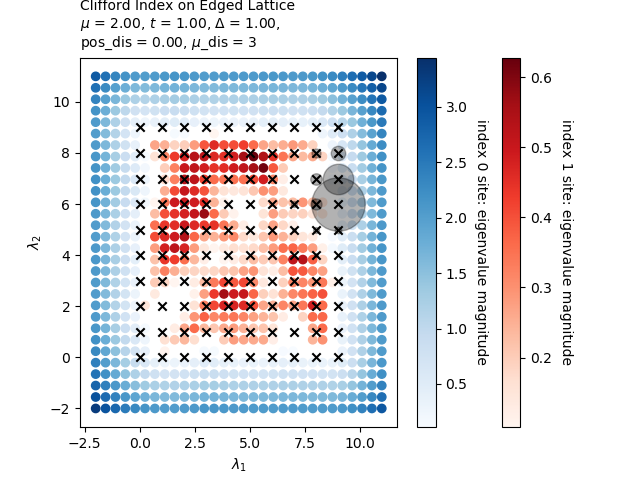
\includegraphics[width=.45\linewidth]{figures/mu_dis_edge/img01.png} }}%

\subfloat{{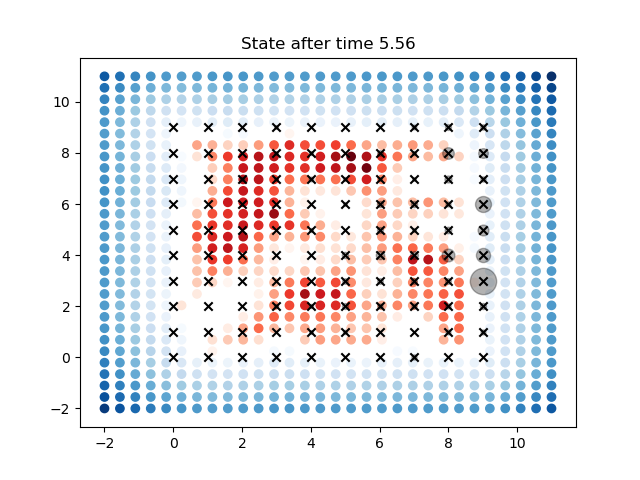
\includegraphics[width=.45\linewidth]{figures/mu_dis_edge/img02.png} }}%
\subfloat{{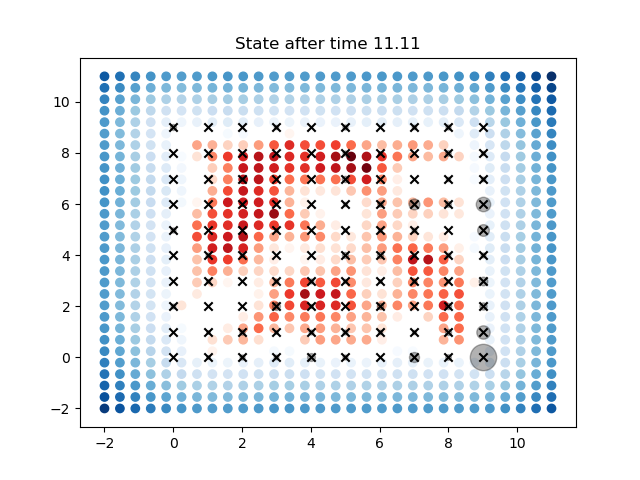
\includegraphics[width =.45\linewidth]{figures/mu_dis_edge/img03.png} }}%

\subfloat{{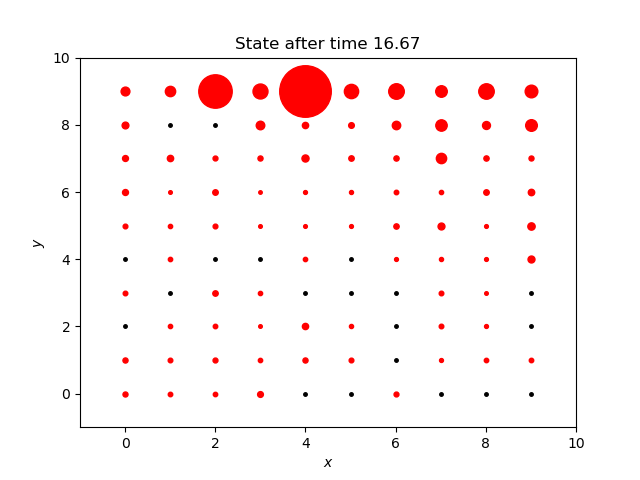
\includegraphics[width =.45\linewidth]{figures/mu_dis_edge/img04.png} }}%
\subfloat{{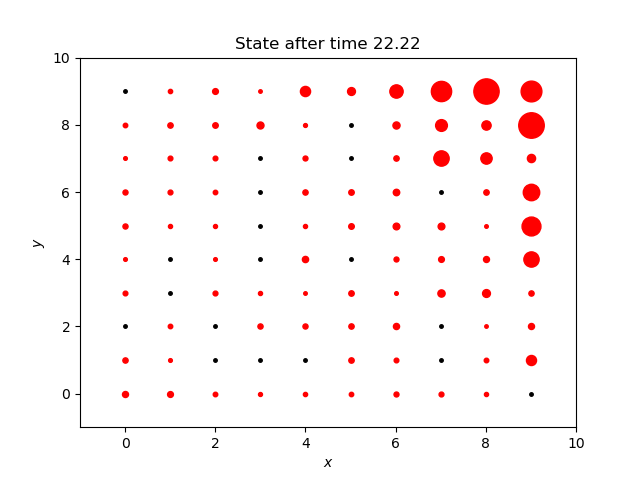
\includegraphics[width=.45\linewidth]{figures/mu_dis_edge/img05.png} }}%

\subfloat{{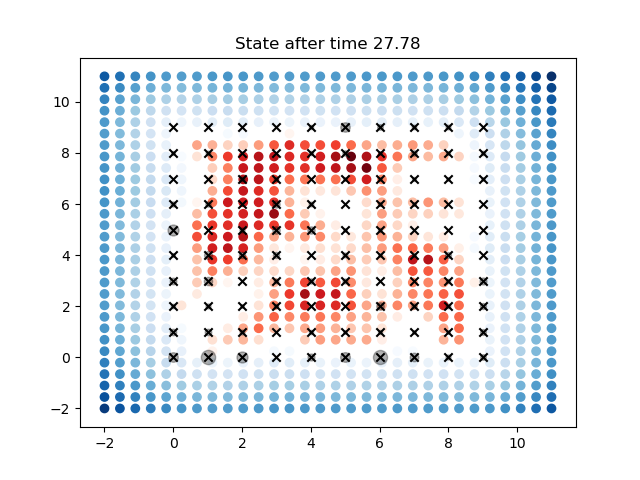
\includegraphics[width=.45\linewidth]{figures/mu_dis_edge/img06.png} }}%
\subfloat{{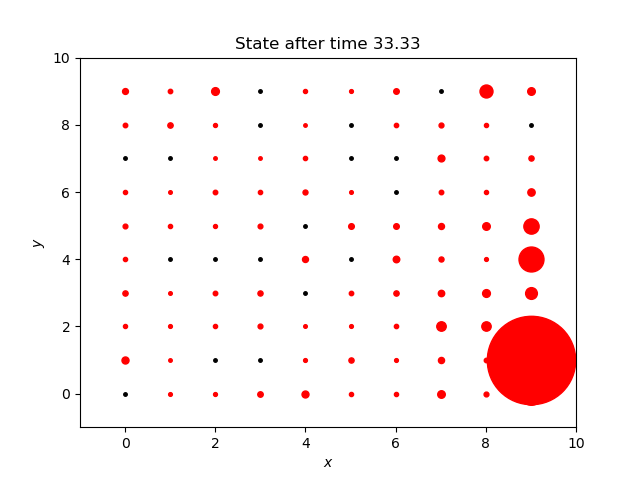
\includegraphics[width =.45\linewidth]{figures/mu_dis_edge/img07.png} }}%
\caption{Propagation on Edge of $p_x + ip_y$ Model with Onsite Disorder: with parameters as in Figure \ref{fig:pxipy_prop}, we now add onsite disorder to the lattice, letting $\mu$ for each site be chosen uniformly at random on $[0.5,3.5]$.
We initialize a state on the edge of the lattice, where there is still a boundary between the index 1 interior and index 0 exterior.
And the state successfully propagates along the edge.
}%
\label{fig:mu_dis_edge_prop}%
\end{figure}

\begin{figure}
\centering
\subfloat{{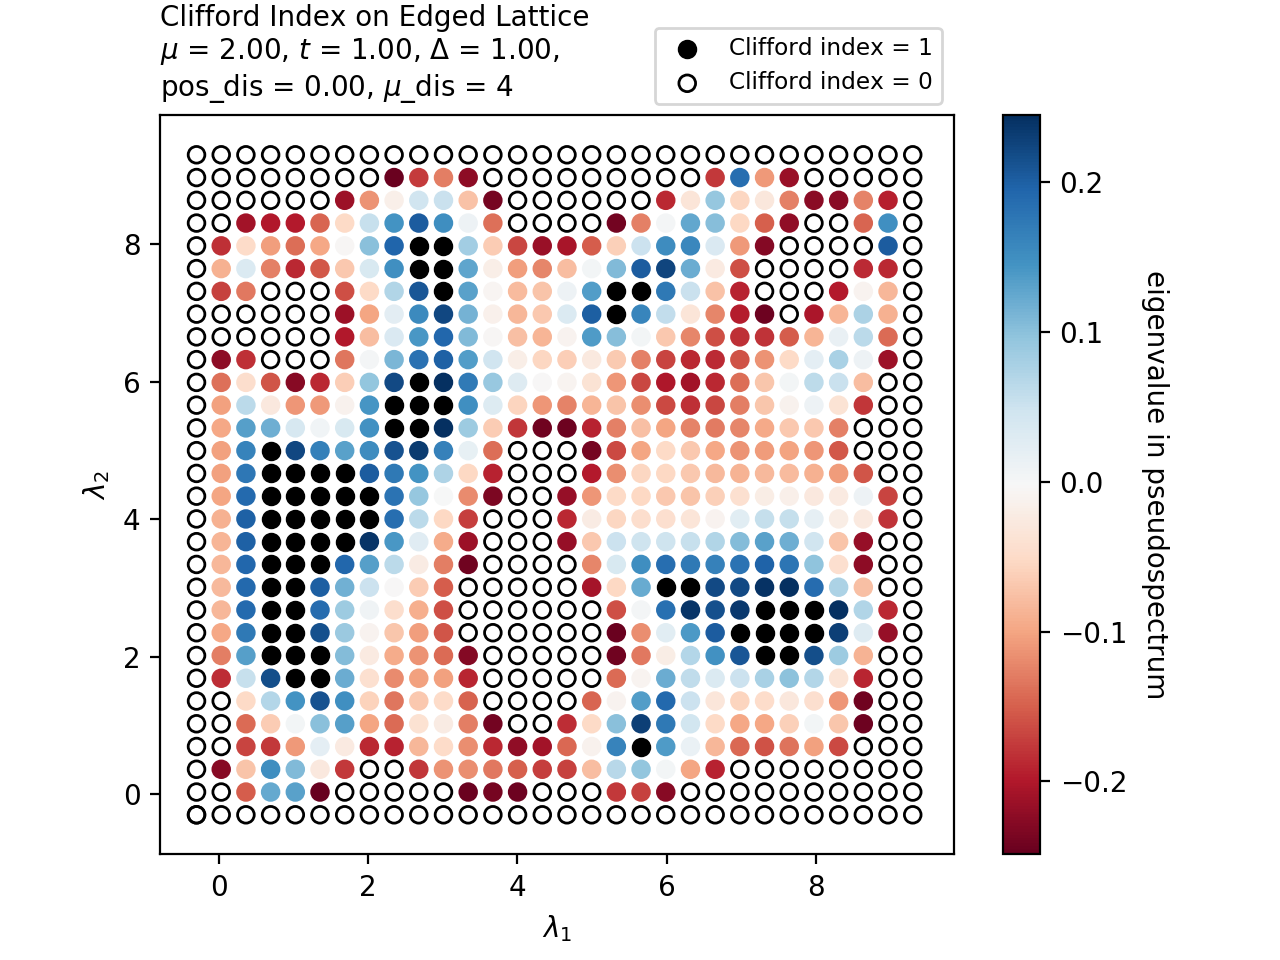
\includegraphics[width=.45\linewidth]{figures/mu_dis_interior/index.png} }}%
\subfloat{{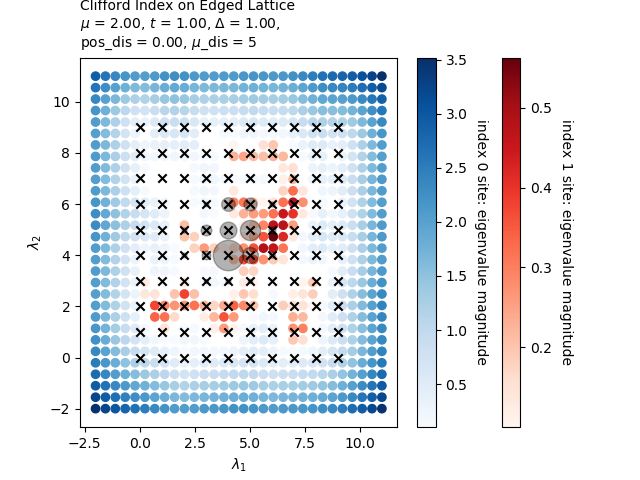
\includegraphics[width=.45\linewidth]{figures/mu_dis_interior/img01.png} }}%

\subfloat{{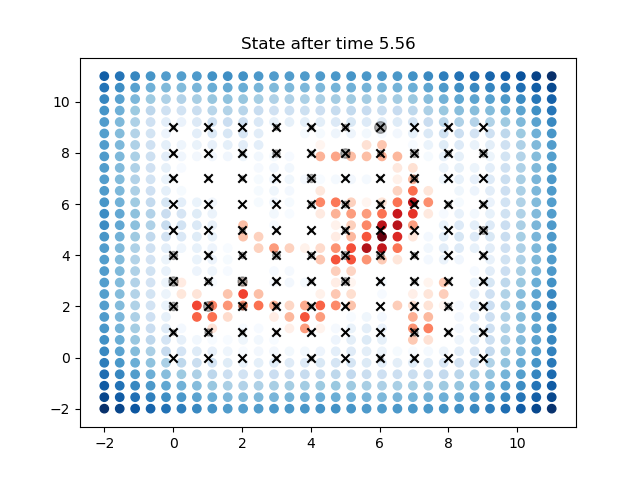
\includegraphics[width=.45\linewidth]{figures/mu_dis_interior/img02.png} }}%
\subfloat{{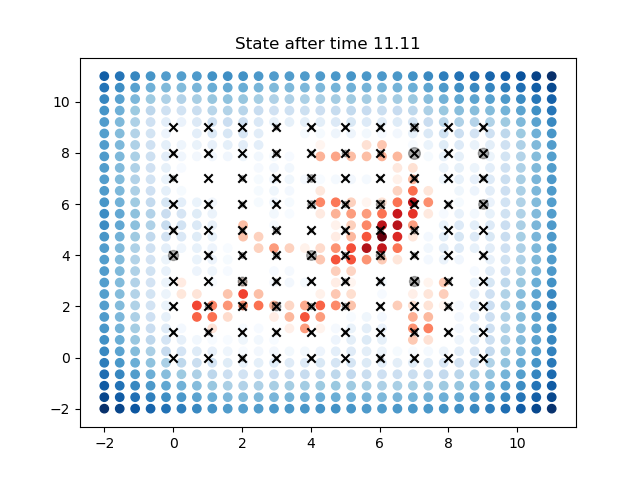
\includegraphics[width =.45\linewidth]{figures/mu_dis_interior/img03.png} }}%

\subfloat{{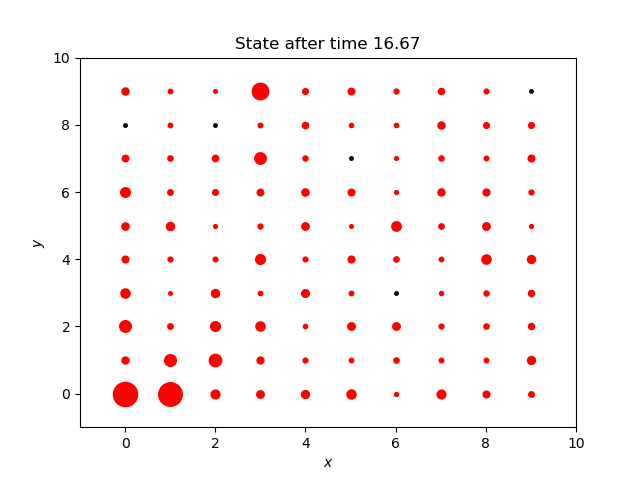
\includegraphics[width =.45\linewidth]{figures/mu_dis_interior/img04.png} }}%
\subfloat{{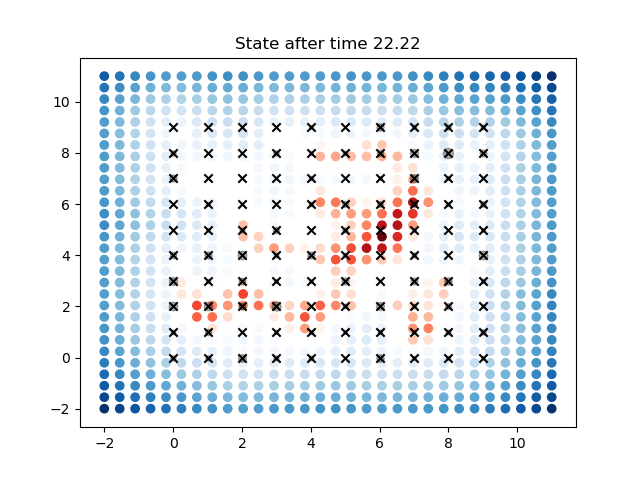
\includegraphics[width=.45\linewidth]{figures/mu_dis_interior/img05.png} }}%

\subfloat{{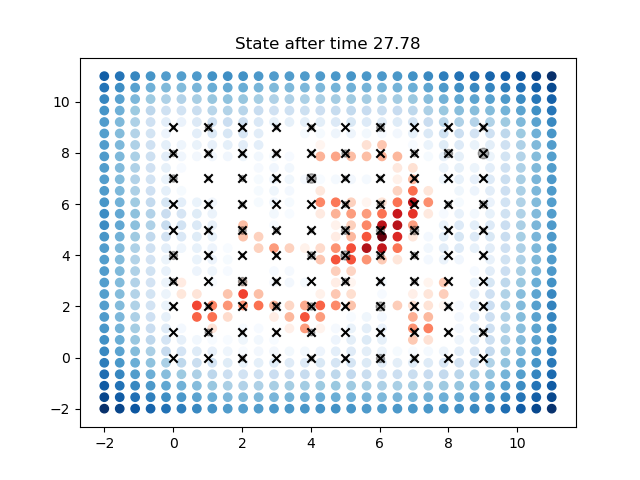
\includegraphics[width=.45\linewidth]{figures/mu_dis_interior/img06.png} }}%
\subfloat{{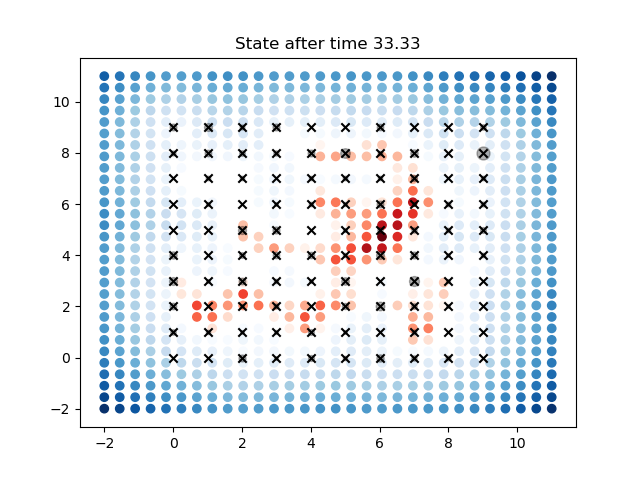
\includegraphics[width =.45\linewidth]{figures/mu_dis_interior/img07.png} }}%
\caption{Propagation on Interior of $p_x + ip_y$ Model with Onsite Disorder: with parameters as in Figure \ref{fig:pxipy_prop}, we now increase disorder, letting $\mu$ for each site be chosen uniformly at random on $[0,4]$.
We do this to obtain regions of both index 1 and 0 in the interior of the lattice.
We initialize a state on the boundary between a region of index 1 on the left and index 0 on the right.
However we do not see continued propagation along the edge of either of the regions.
We believe this is because the eigenvalue magnitudes are changing gradually across the boundary, rather than abruptly as in Figures \ref{fig:pxipy_prop},  \ref{fig:pos_dis_prop}, and \ref{fig:mu_dis_edge_prop}.
}%
\label{fig:mu_dis_interior_prop}%
\end{figure}

\aw{This is a good ordering of things.}

\section{Future Work}

\section{Notes from Monday Meeting}

\printbibliography

\end{document}
